\documentclass[12pt]{article}
\usepackage{preamble}

\pagestyle{fancy}
\fancyhead[LO,LE]{Дополнительные главы \\ высшей математики}
\fancyhead[RO,RE]{Лекции Далевской О. П.}

\fancyfoot[L]{\scriptsize исходники найдутся тут: \\ \url{https://github.com/pelmesh619/itmo_conspects} \Cat}

\renewcommand{\thesection}{}

\begin{document}

    \tableofcontents
    \clearpage

    % begin addchapters2_2025_02_07.tex





\section{1. Основные понятия}

\subsection{1.1. Комплексное число}

\Mem $\Complex = \{ (a, b) \ | \ a, b \in \Real\}$

Обозначение: $z = (a, b) = a + bi$, где $i = (0, -1) = \sqrt{-1}$

\underline{Основные операции}:

\begin{enumerate}
    \item $\RE z = a$ - вещественная часть, $\IM z = b$ - мнимая часть
    \item $z_1 + z_2 = (a_1, b_1) + (a_2, b_2) = (a_1 + a_2, b_1 + b_2) = (a_1 + a_2) + i(b_1 + b_2)$
    \item $z_1 \cdot z_2 = (a_1 + b_1 i) * (a_2 + b_2 i) = (a_1 a_2 - b_1 b_2) + i (a_1 b_2 + a_2 b_1)$
    \item $z^n = \rho^n (\cos n\varphi + i \sin n\varphi)$ - \textbf{формула Муавра}, где $\rho = |z|, \varphi = \arg z$
    \item $\sqrt[n]{z} = \sqrt[n]{\rho} \left(\cos \frac{\varphi + 2\pi k}{n} + i \sin \frac{\varphi + 2\pi k}{n}\right)$, где $\rho = |z|, \varphi = \arg z, k \in \Integer$
    \item При $n = 2$ $\sqrt{z} = \sqrt{a + bi} = \pm (c + di)$, 
        где $c = \sqrt{\frac{a + \sqrt{a^2 + b^2}}{2}}, d = \operatorname{sign}(b) \sqrt{\frac{-a + \sqrt{a^2 + b^2}}{2}}$
\end{enumerate}

\begin{minipage}{\textwidth}
    % https://www.geogebra.org/calculator/xjg67fnv

    \begin{wrapfigure}{r}{0pt}
        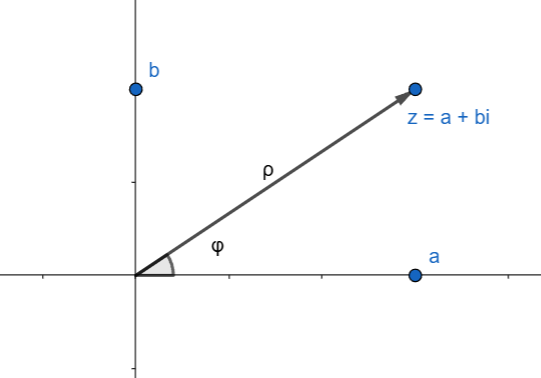
\includegraphics[width=7cm]{addchapters2/images/addchapters2_2025_02_07_6}
    \end{wrapfigure}

    Тригонометрическая форма:

    $z = a + bi = \rho (\cos \varphi + i \sin \varphi)$, где $\rho = |z| = \sqrt{a^2 + b^2}, \varphi = \arg z \in [0; 2\pi)$

    $\Arg z = \arg z + 2\pi k, k \in \Integer$

    По формуле Эйлера $z = \rho (\cos \varphi + i \sin \varphi) = \rho e^{i \varphi}$
\end{minipage}

\subsection{1.2. Комплексная плоскость}

\Def Окрестность точки $z_0 \in \Complex$ определяется как $U_\delta (z_0) = \{z \in \Complex \ \Big| \ |z - z_0| < \delta\}$

Тогда $\overset{\circ}{U}_\delta (z_0) = U_\delta (z_0) \setminus \{ z_0 \}$ - выколотая окрестность

\Def Для данной множества точек $A$ точка $z_0$ считается

\begin{itemize}
    \item внутренней, если для любого $\delta$ $U_\delta (z_0) \subset A$
    \item граничной, если для любого $\delta$ $\exists z \in U_\delta (z_0) \Big| z \in A$ и $\exists z \in U_\delta (z_0) \Big| z \notin A$
\end{itemize}

\Def Открытое множество состоит только из внутренних точек

\Defs Закрытое множество содержит все свои граничные точки

\Defs Границой $\Gamma_D$ (иногда обозн. $\delta D$) для множества $D$ называют множество всех граничных точек $D$

\Defs Если любые две точки множества можно соединить ломаной линией конечной длины, то множество считается связным

\Defs Множество $D \subset \Complex$ называется областью, если $D$ - открытая и связная

\Defs Кривая $l \subset \Complex$ считается непрерывной, если $l = \{z \in \Complex \ | \ z = \varphi(t) + i \psi(t), t \in \Real\}$, где $\varphi(t), \psi(t)$ - непрерывные функции

\Notas Если $\varphi(t)$ и $\psi(t)$ дифференцируемы и их производные непрерывные, то кривая $l$ гладкая

\Defs Непрерывная замкнутая (то есть начальная и конечная точки совпадают) без самопересечений кривая называется контуром

\Notas Односвязную область можно стянуть в точку

% https://www.geogebra.org/calculator/nhbjhbag

\begin{multicols}{2}
    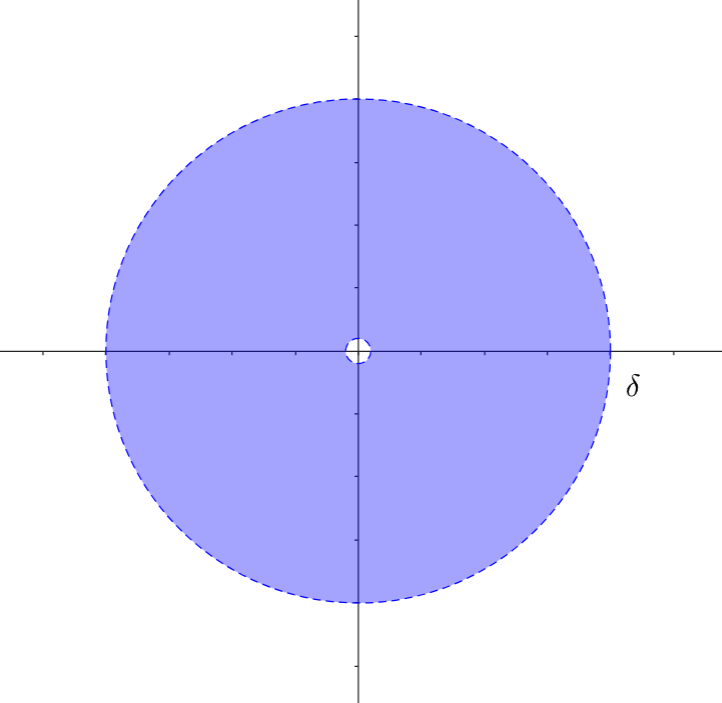
\includegraphics[width=0.4\textwidth]{addchapters2/images/addchapters2_2025_02_07_1}

    \ExNs{1} $D = \{z \in \Complex \ \Big| \ 0 < |z| < \delta\}$ - область связаная, но не односвязная, ее нельзя стянуть из-за дырки

    \mediumvspace

    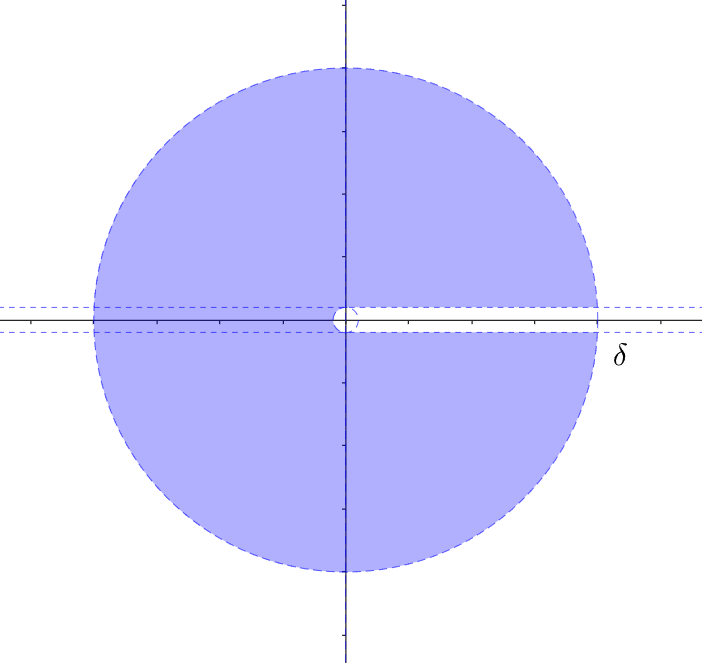
\includegraphics[width=0.4\textwidth]{addchapters2/images/addchapters2_2025_02_07_2}

    \ExN{2} $D = \{z \in \Complex \ \Big| \ 0 < |z| < \delta, \arg z \neq 0\}$ - область связная и односвязная
\end{multicols}

\begin{multicols}{2}
    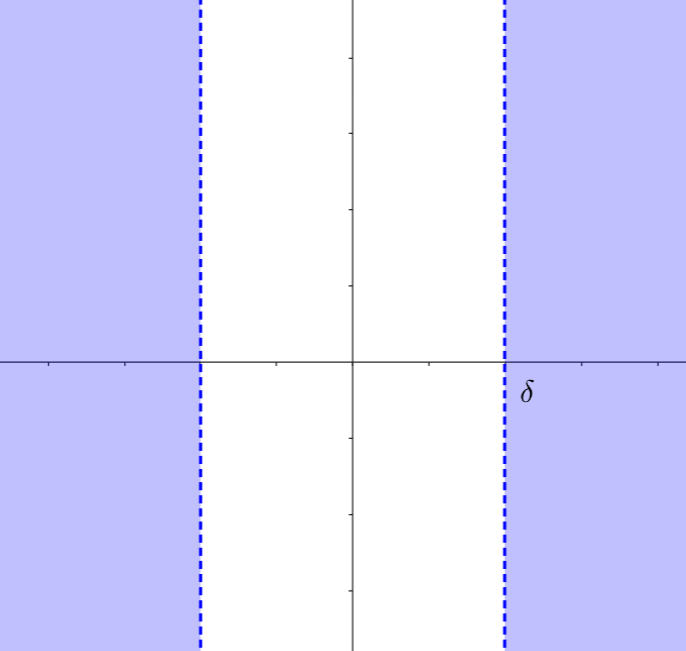
\includegraphics[width=0.4\textwidth]{addchapters2/images/addchapters2_2025_02_07_3}

    \ExN{3} $D = \{z \in \Complex \ \Big| \ |\RE z| < \delta\}$ - несвязная область

    \mediumvspace

    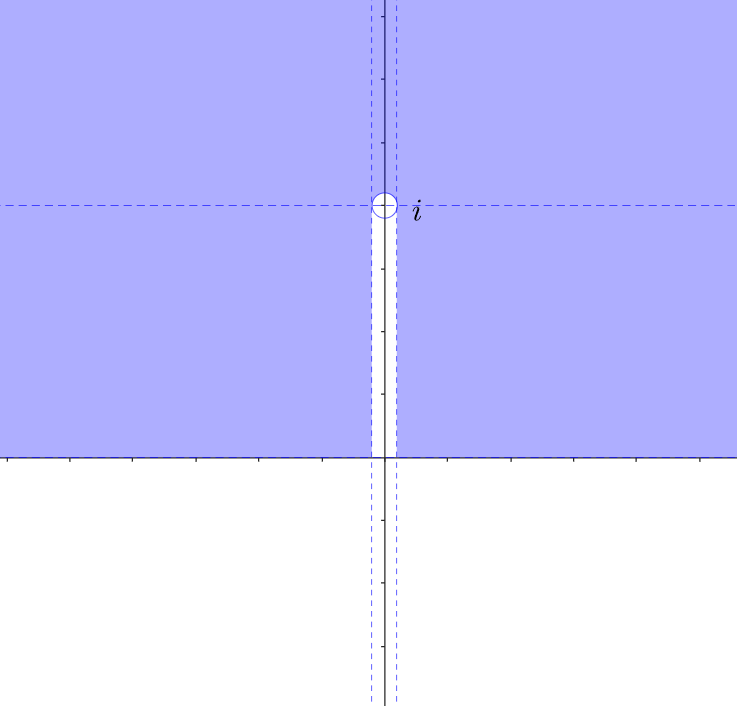
\includegraphics[width=0.4\textwidth]{addchapters2/images/addchapters2_2025_02_07_4}

    \ExN{4} $D = \{z \in \Complex \ \Big| \ \IM z \geq 0, z \notin [0, i]\}$ - здесь под $[0, i]$ подразумевается линейный отрезок на оси
\end{multicols}

\Nota Дальше все рассматриваемые $\Gamma_D$ будут состоять из кусочногладких и изолированных кривых

\subsection{1.3. Предел}

\Mem Последовательность $\{z_n\} = z_1, z_2, z_3, \dots, z_n, \dots$

\Def Пределом $\{z_n\}$ называют число $z$ такое, что

$\forall \varepsilon > 0 \ \exists \underset{n_0 = n_0(\varepsilon)}{n_0 = \Natural} \ \Big| \ \forall n > n_0 \ |z_n - z| < \varepsilon$

Обозначается $\lim_{n \to \infty} z_n = z$

\Nota $\{z_n\}$ можно представить как ${x_n + i y_n}$, то есть двумя $\Real$-последовательностями

\begin{MyTheorem}
    \Ths $\exists \lim_{n \to \infty} z_n = \underset{x, y \in \Real}{x + i y} \Longleftrightarrow $
    \begin{tabular}{l} $\exists \lim_{n \to \infty} x_n = \lim_{n \to \infty} \RE z_n = x$ \\ $\exists \lim_{n \to \infty} y_n = \lim_{n \to \infty} \IM z_n = y$ \end{tabular}
\end{MyTheorem}

\begin{MyProof}
    \fbox{$\Longleftarrow$} $\forall \varepsilon > 0 \ \exists \underset{n_0 = \max (n_{0x}, n_{0y})}{n_0 \in \Natural} \ \Big| \ \forall n > n_0 \begin{tabular}{l} |x_n - x| < \frac{\varepsilon}{2} \\ |y_n - y| < \frac{\varepsilon}{2} \end{tabular}$
    
    $|z_n - z| = |(x_n - x) + i(y_n - y)| \leq |x_n - x| + |y_n - y| < \frac{\varepsilon}{2} + \frac{\varepsilon}{2}$

    То есть $\forall \varepsilon > 0 \dots |z_n - z| < \varepsilon$

    \fbox{$\Longrightarrow$} $\forall \varepsilon > 0 \ |z_n - z| = |(x_n - x) + i(y_n - y)| < \varepsilon \Longrightarrow 
    \begin{cases}
        |x_n - x| \leq |(x_n - x) + i(y_n - y)| < \varepsilon \\
        |y_n - y| \leq |(x_n - x) + i(y_n - y)| < \varepsilon \\
    \end{cases} \Longrightarrow \exists \lim_{n \to \infty} x_n = x$ и $\exists \lim_{n \to \infty} y_n = y$

\end{MyProof}

\Nota Для комплексных чисел работают теоремы для пределов (сумма пределов, произведение пределов и т.д.), критерий Коши и другие

\Def $\lim_{n \to \infty} z_n = \infty \Longleftrightarrow \forall \varepsilon > 0 \ \exists \underset{n_0 = n_0(\varepsilon)}{n_0 \in \Natural} \ \Big| \ n > n_0 \ |z| > \varepsilon$

\Defs Точка $z$, определенная как предел, равный $\infty$, называется бесконечно удаленной. Но существует множество последовательностей, чьи пределы удаляются на бесконечность разными путями на плоскости

\Def Стереографическая проекция (сфера Римана)

% https://www.geogebra.org/calculator/kjesw2gx

\begin{center}
    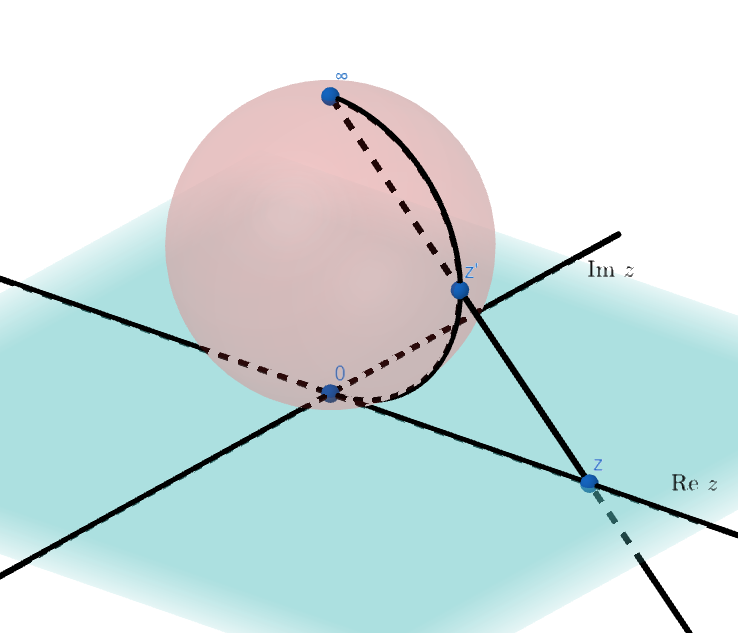
\includegraphics[width=0.55\textwidth]{addchapters2/images/addchapters2_2025_02_07_5}
\end{center}

Поместим сферу на комплексную плоскость и сделаем биекцию точек плоскости на точки сферы: проведем из верхней точки сферы лучи вниз на плоскость, и точка, где луч пересекает сфера,
будет считаться отображением для данной точки. Заметим, что в этом случае бесконечно удаленные точки будут отображаться в верхнюю точку сферы

\Def $\Complex \cup \{\infty\} = \overline{\Complex}$ - расширенная комплексная плоскость

Однако $z + \infty$ не определена, $\infty + \infty$ не определена. 
Но $\infty = \lim_{n \to \infty} \frac{1}{z_n}$ при $z_n \underset{n \to \infty}{\longrightarrow} 0$; $\infty = \infty \cdot \lim_{n \to \infty} z_n$ при $z_n \longrightarrow z$

Записью $[-\infty; +\infty]$ обозначается ось $\overline{\Real}$; 

\qquad\qquad $[-i\infty; +i\infty]$ - мнимая расширенная ось

Путь $x \pm i \infty$ при фикс. $x$ - вертикальная прямая; 

\qquad\qquad $iy \pm \infty$ - горизонтальная прямая; 

\qquad\qquad $e^{i\varphi} \cdot \infty$ - прямая, проходящая через начало координат



% end addchapters2_2025_02_07.tex

% begin addchapters2_2025_02_21.tex





\section{2. Комплексная функция}

\hypertarget{complex_function}{}

\subsection{2.1. Определение}

\Mem $f : E \subset \Real \longrightarrow D \subset \Real \ \overset{def}{\Longleftrightarrow} \ $ отображение такое, 
что $\forall x \in E \ \exists! y \in D \ | \ y = f(x)$

\Def $f : D \subset \Complex \longrightarrow G \subset \Complex \ \overset{def}{\Longleftrightarrow} \ $ отображение такое, 
что $\forall z \in D \ \exists w \in G \ | \ f(z) = w$

\Defs Если $\forall z \in D \ \exists! w \in G$, то $f$ называется однозначной функцией

\Defs Если $\forall z_1, z_2 \in D (z_1 \neq z_2) \Longrightarrow f(z_1) \neq f(z_2)$, 
то $f$ называется однолистной функцией

\ExN{1} $w = \sqrt{z}$ - неоднозначная функция

$\letsymbol z = 1 = 1 (\cos 0 + i \sin 0)$

$\sqrt{z} = \sqrt{1} \left(\cos \frac{2\pi k}{2} + i \sin \frac{2\pi k}{2}\right)$

$w_1 = 1, \quad w_2 = -1$

\ExN{2} $w = z^2$ - неоднолистная функция

$z_1 = 1, z_2 = -1 \qquad\qquad w(z_1) = w(z_2) = 1$

\Nota Если $f(z)$ однозначна и однолистна, то $f(z)$ - взаимно однозначное соответствие (биекция). Тогда $\exists g(x) \ | \ g(f(x)) = x$

Комплексную функцию $f(z)$ можно представить как $u(x, y) + i v(x, y)$, где $x + iy = z$

\Ex $w = z^2 = (x + iy)^2 = x^2 + 2ixy - y^2 = (x^2 - y^2) + i \cdot 2xy$

$u(x, y) = (x^2 - y^2), \qquad\qquad v(x, y) = 2xy$

\subsection{2.2. Предел функции}

\hypertarget{complex_limit}{}

\Def $L \in \Complex, f : D \longrightarrow G, \quad L \overset{def}{=} \lim_{z \to z_0} f(z) \Longrightarrow
\forall \varepsilon > 0 \ \exists \underset{\delta = \delta(\varepsilon)}{\delta > 0} \ \Big| \ z \in D, z \in \overset{\circ}{U}_\delta(z_0) \ f(x) \in U_\varepsilon(L)$

В определении существование и значение $L$ не должно зависеть от пути, по которому $z$ приближается к точке сгущения $z_0$.
Может быть так, что для любого направления стремления предел есть, но в общем смысле не существует

% https://www.geogebra.org/calculator/hgk25mjs

\begin{wrapfigure}{R}{0pt}
    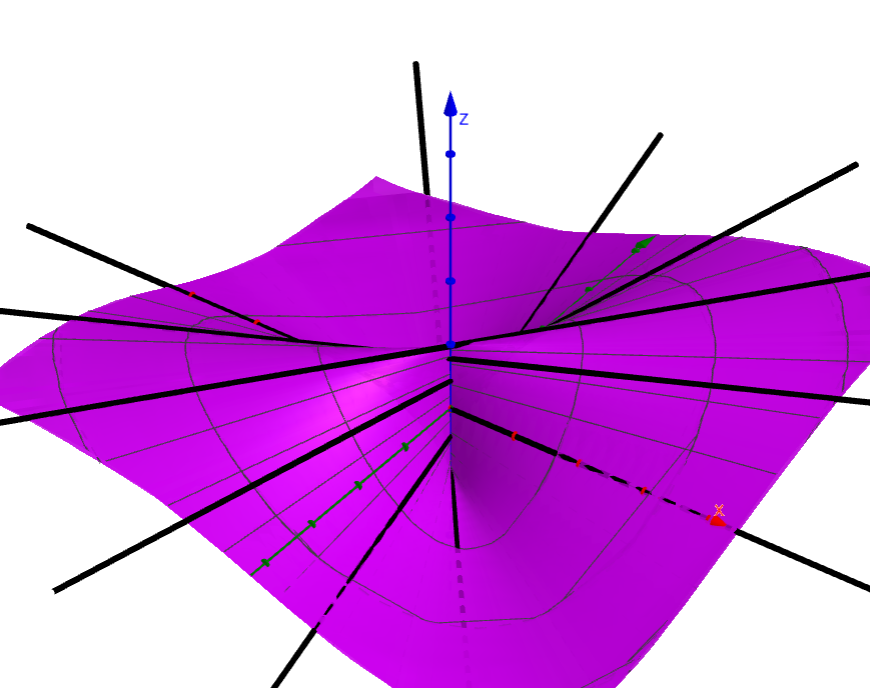
\includegraphics[width=7cm]{addchapters2/images/addchapters2_2025_02_21_2}
\end{wrapfigure}

\Ex $f(z) = \frac{1}{2i} \left(\frac{z}{\overline{z}} - \frac{\overline{z}}{z}\right) \qquad\qquad \letsymbol z = \rho e^{i\varphi}$

$f(z) = \frac{1}{2i} \left(\frac{\rho e^{i\varphi}}{\rho e^{-i\varphi}} - \frac{\rho e^{-i\varphi}}{\rho e^{i\varphi}}\right) =
\frac{1}{2i} \left(e^{2i\varphi} - e^{-2i\varphi}\right) = \frac{1}{2i} (\cos 2\varphi + i\sin 2\varphi - \cos 2\varphi + i\sin 2\varphi) = \sin 2\varphi$

Зафиксируем $\varphi = \varphi^* \in [0; 2\pi)$, тогда $\sin 2\varphi^* \in [-1; 1]$

$\lim_{z \to 0} f(z) = \lim_{\substack{\rho \to 0 \\ \varphi = \varphi^*}} f(z) = 
\lim_{\substack{\rho \to 0 \\ \varphi = \varphi^*}} \sin 2\varphi = \sin 2\varphi^* \in [-1; 1]$

Значения предела занимает отрезок $[-1; 1] \Longrightarrow \not\exists \lim_{z \to 0} f(z)$

На рисунке изображена $\sin 2\varphi$, на оси $Oz$ изображена $\RE w$. Черные линии - это возможные пути приближения $z$ к $0$

\Nota Путь следования предела аналогичен левостороннему и правостороннему пределами $\Real$-функций

\hypertarget{continuity}{}

\DefN{Непрерывность функций в точке $z_0$}

$f : D \longrightarrow G, z_0 \in D$, $f(z)$ называется непрерывной в $z_0$, если $\lim_{z \to z_0} f(z) = f(z_0)$

На языке приращений: $\Delta f = f(z_0 + \Delta z) - f(z_0) \underset{\Delta z \to 0}{\longrightarrow} 0$

$\Delta z = z - z_0 = \Delta x + i \Delta y \to 0 \Longrightarrow 
\begin{cases}\Delta x \to 0 \\ \Delta y \to 0\end{cases} \Longrightarrow 
\Delta \rho \to 0$

\subsection{2.3. Элементарные комплексные функции}

\hypertarget{elementary_functions}{}

\ExN{1} Линейная $f(z) = az + b, \qquad\qquad a, b \in \Complex \quad a \neq 0$

Эта функция однозначная, однолистная $\Longrightarrow \exists f^{-1}(z) = g(z) = \frac{z - b}{a}$

\underline{Геометрический смысл}:

$a \in \Complex, z \in \Complex$

$az = |a| |z| (\cos (\varphi_a + \varphi_z) + i \sin (\varphi_a + \varphi_z))$ - поворот и растяжение 
($\varphi_a = \arg a$, $\varphi_z = \arg z$)

$az + b = (x_{az} + x_b) + i (y_{az} + y_b)$ - сдвиг

То есть линейная функция - композиция из поворота, растяжения и сдвига

\ExN{2} Степенная $w = z^n, \quad n \in \Natural$ - однозначная, может быть неоднолистной

Для $n \in \Rational$ функция становится неоднозначной

\Exs $w = z^2 \qquad\qquad z = \rho e^{i\varphi}, w = \rho^2 e^{2i\varphi}$

Пусть $z_1 \neq z_2$ и $w(z_1) = w(z_2)$, тогда $\arg z_1 = \arg z_2 \pm \pi$ 

$w(z_1) = \rho^2 e^{2i\arg z_1} = \rho^2 e^{2i (\arg z_1 + 2\pi k)}$

$w(z_2) = \rho^2 e^{2i\arg z_2} = \rho^2 e^{2i (\arg z_1 + \pi)} = \rho^2 e^{i (2\arg z_1 + 2\pi)} = w(z_1)$

Область однолистности $z^2$ - множество точек, для которых $\arg z \in [0; \pi)$

Точку $w = 0$ называют точкой разветвления

% https://www.geogebra.org/calculator/phuam9sh

\begin{wrapfigure}{r}{0pt}
    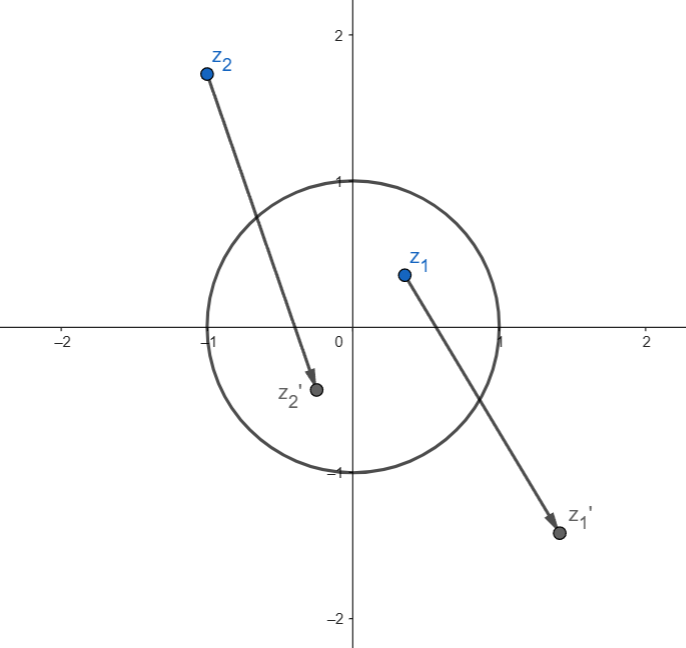
\includegraphics[width=7cm]{addchapters2/images/addchapters2_2025_02_21_1}
\end{wrapfigure}

\Exs $w = z^{-1} = \frac{1}{z} \qquad\qquad w(0) = \infty, w(\infty) = 0$

$z \in \Complex \setminus \{0\}$ - функция обратима

$w = re^{i\psi} = \frac{1}{\rho e^{i\phi}} = \frac{1}{\rho} e^{-i\varphi} \Longrightarrow |w| = \frac{1}{|z|}, \arg w = -\arg z$

Преобразование $|w| = \frac{1}{|z|}$ называется инверсией, а $\arg w = -\arg z$ дает симметрию относительно $\RE z$

\ExN{3} Рациональная $f(z) = \frac{P_n(z)}{Q_m(z)}, \qquad\qquad n, m \in \Natural$

\ExN{4} Показательная $w = e^z = e^x \cdot e^{iy} = e^x (\cos y + i \sin y)$

\underline{Свойства}: 

\begin{enumerate}
    \item $e^{z_1 + z_2} = e^{z_1} \cdot e^{z_2}$
    \item $\left(e^{z_1}\right)^{z_2} = e^{z_1 z_2}$
    \item $e^{z + 2\pi i} = e^{z} \cdot e^{2\pi i} = e^z$ - показательная функция периодична с периодом $2\pi i$
\end{enumerate}

\ExN{5} Логарифмическая $w = \Ln z$

Если $e^w = e^{u + vi} = e^u (\cos v + i \sin v) = z = |z| e^{i\arg z}$, то $u = \ln |z|$, $v = \arg z + 2\pi k$

Тогда \fbox{$\Ln z = \ln |z| + i (\arg z + 2\pi k)$}

$\ln z = \Ln z$ при $k = 0$ - т. н. главное значение




% end addchapters2_2025_02_21.tex

% begin addchapters2_2025_03_07.tex





Заметим, что $w = e^z = e^x (\cos y + i \sin y)$ - многолистная функция, а $w = \Ln z = \ln \rho + i (\arg z + 2\pi k)$ - многозначная

\ExN{6} Тригонометрические и гиперболические

\begin{multicols}{2}
    \begin{center}
        $\sin z = \frac{e^{iz} - e^{-iz}}{2i}$

        $\cos z = \frac{e^{iz} + e^{-iz}}{2}$

        $\sh z = \frac{e^{z} - e^{-z}}{2}$

        $\ch z = \frac{e^{z} + e^{-z}}{2}$
    \end{center}
\end{multicols}

\Nota Рассмотрим уравнение $\sin z = A \in \Complex$

$\frac{e^{iz} - e^{-iz}}{2i} = A \Longrightarrow e^{2iz} - 2iAe^{iz} - 1 = 0$

При $t = e^{iz}$ получаем квадратное уравнение, у которого в $\Complex$ всегда будет два корня. 
Это значит, что в $\Complex$ $\sin$ и $\cos$ принимают любые значения (то есть $|\sin z| > 1$)

\subsection{2.4. Дифференцирование ФКП}

\Def $w = f(z), w : D \subset \Complex \longrightarrow \Complex, z_0 \in D$. \textbf{Производная} функции
$w(z_0)$ - это предел $\lim_{\Delta z \to 0} \frac{f(z_0 + \Delta z) - f(z_0)}{\Delta z} = \lim_{\Delta z \to 0} \frac{\Delta f}{\Delta z}$, 
если он существует и не зависит от пути $z \to z_0$

\Mem Дифференцирование $y = f(x)$:

\begin{tabular}{ll}
    В Ф$_1$П: & $\Delta y = f(x_0 + \Delta x) - f(x_0) \underset{A \in \Real}{=} A\Delta x + o(\Delta x)$ \\
    В Ф$_2$П: & $\Delta f = f(x_0 + \Delta x, y_0 + \Delta y) - f(x_0, y_0) = A\Delta x + B \Delta y + \alpha_1 + \alpha_2 = 
    \frac{\partial f}{\partial x} \Delta x + \frac{\partial f}{\partial y} \Delta y + o(\Delta x) + o(\Delta y)$
\end{tabular}

\hypertarget{derivative}{}

\Def $f(z)$ называется дифференцируемой в точке $z_0$, если $\exists f^\prime(z_0) \in \Complex$

\Defs Дифференцируемая в точке $z_0$ функция $w = f(z)$, производная $f^\prime(z_0)$ которой непрерывна в $z_0$,
называется аналитической (или аналитичной) функцией в $z_0$

\hypertarget{cauchy_riemann}{}

\begin{MyTheorem}
    \Ths Критерий аналитичности (или Условие Коши-Римана)

    \begin{center}
        $f(x) = u(x, y) + i v(x, y)$ аналитична в точке $z_0 = x + iy$ 
        
        \rotatebox{90}{$\Longleftrightarrow$}
    
        $\exists \frac{\partial u}{\partial x}, \frac{\partial u}{\partial y}, \frac{\partial v}{\partial x}, \frac{\partial v}{\partial y}$ непрерывны в $z$ и
        $\begin{cases}\frac{\partial u}{\partial x} = \frac{\partial v}{\partial y} \\ \frac{\partial u}{\partial y} = -\frac{\partial v}{\partial x}\end{cases}$
    \end{center}

    Причем, $f^\prime(z) = u_x + i v_x = v_y - i u_y = u_x - i u_y = v_y + i v_x$
\end{MyTheorem}

\begin{MyProof}
    \fbox{\Longrightarrow} \ $f$ аналитическая в $z$ $\Longleftrightarrow \exists$ непрерывная 
    $f^\prime(z) = \\ = \lim_{\Delta z \to 0} \frac{\Delta f}{\Delta z} = [\text{предел не зависит от пути}] = 
    \lim_{\Delta x \to 0} \frac{f(x + \Delta x, y) - f(x, y)}{\Delta x} = \\
    = \lim_{\Delta x \to 0} \frac{u(x + \Delta x, y) + i v(x + \Delta x, y) - u(x, y) - v(x, y)}{\Delta x} = \\
    = \lim_{\Delta x \to 0} \left(\frac{u(x + \Delta x, y) - u(x, y)}{\Delta x} + i \frac{v(x + \Delta x, y) - v(x, y)}{\Delta x}\right) = \\
    = \lim_{\Delta x \to 0} \left(\frac{\Delta_x u}{\Delta x} + i \frac{\Delta_x v}{\Delta x}\right) = 
    \lim_{\Delta x \to 0} \frac{\Delta_x u}{\Delta x} + i \lim_{\Delta x \to 0} \frac{\Delta_x v}{\Delta x} = 
    \frac{\partial u}{\partial x} + i \frac{\partial v}{\partial x} = u_x + i v_x$

    Аналогично при $i \Delta y \to 0$ получаем $\lim_{\Delta y \to 0} \frac{f(x, y + \Delta y) - f(x, y)}{i \Delta y} = \\
    = \lim_{\Delta y \to 0} \left(\frac{u(x, y + \Delta y) - u(x, y)}{i \Delta y} + \frac{v(x, y + \Delta y) - v(x, y)}{\Delta y}\right) = 
    \lim_{\Delta y \to 0} \frac{\Delta_y v}{\Delta y} - i \lim_{\Delta y \to 0} \frac{\Delta_y u}{\Delta y} = 
    v_y - i u_y$

    Итак, $f^\prime(z) = u_x + i v_x = v_y - i u_y$

    Отсюда $u_x = v_y$ и $u_y = -v_x$

    \mediumvspace 

    \fbox{\Longleftarrow} \ $\exists$ непрерывные $u_x, u_y, v_x, v_y \Longleftrightarrow u(x, y), v(x, y)$ 
    дифференцируемы в $(x, y)$, тогда $\Delta u = u_x \Delta x + u_y \Delta y + \alpha_1 (x, y, \Delta x, \Delta y) + 
    \alpha_2 (x, y, \Delta x, \Delta y)$

    $\alpha_1 = o(\Delta \rho), \quad \Delta \rho = (\Delta x)^2 + (\Delta y)^2$

    $\Delta v = v_x \Delta x + v_y \Delta_y + \beta_1 + \beta_2$

    $\Delta f = u(x + \Delta x, y + \Delta y) + iv(x + \Delta x, y + \Delta y) - (u(x, y) + i v(x, y)) = 
    u_x \Delta x + u_y \Delta y + \alpha + i(v_x \Delta x + v_y \Delta y + \beta)$

    $\frac{\Delta f}{\Delta z} = \frac{u_x \Delta x + u_y \Delta y + i v_x \Delta x + i v_y \Delta y}{\Delta x + i \Delta y} + 
    \frac{\alpha + i \beta}{\Delta x + i \Delta y} = \frac{u_x(\Delta x + i \Delta y)}{\Delta x + i \Delta y} + 
    \frac{v_x(i \Delta x - \Delta y)}{\Delta x + i \Delta y} + \frac{\alpha + i\beta}{\Delta x + i \Delta y} = 
    u_x + v_x i + \frac{\alpha + i \beta}{\Delta x + i \Delta y}$

    Тогда $\lim_{\Delta z \to 0} \frac{\Delta f}{\Delta z} = 
    u_x + i v_x + \lim_{\substack{\Delta x \to 0 \\ \Delta y \to 0}} \frac{\alpha + i \beta}{\Delta x + i \Delta y} = 
    u_x + i v_x \Longleftrightarrow f^\prime = u_x + i v_y$, существует и непрерывна в $(x, y)$
\end{MyProof}

\Nota Используя Условие Коши-Римана, получим равенство $u_x + i v_x = v_y - i u_y = u_x - i u_y = v_y + i v_x$

\Notas Коши-Риман в ПСК:

\begin{cases}
    \frac{\partial u}{\partial \rho} = \frac{1}{\rho} \frac{\partial v}{\partial \varphi} \\
    \frac{\partial u}{\partial \varphi} = -\frac{1}{\rho} \frac{\partial v}{\partial \rho}
\end{cases}

Тогда $f^\prime(z) = \frac{1}{z} \left(\frac{\partial v}{\partial \varphi} - i \frac{\partial u}{\partial \varphi}\right) = \frac{\rho}{z} \left(\frac{\partial u}{\partial \rho} + i \frac{\partial v}{\partial \rho}\right)$

\begin{MyProof}
    $u_\rho = u_x \frac{\partial x}{\partial \rho} + u_y \frac{\partial y}{\partial \rho} = u_x \cos \varphi + u_y \sin \varphi$

    $v_\varphi = v_x \frac{\partial x}{\partial \varphi} + v_y \frac{\partial y}{\partial \varphi} = 
    -\rho v_x \sin \varphi + \rho v_y \cos \varphi = \rho u_y \sin \varphi + \rho u_x \cos \varphi = \rho u_\rho$

    \Lab $\frac{\partial u}{\partial \varphi} = -\frac{1}{\rho} \frac{\partial v}{\partial \rho}$
\end{MyProof}

\mediumvspace

\hypertarget{analytic_function_properties}{}

\underline{Свойства аналитических функций}

Пусть $f, g$ - аналитические функции, тогда:

\begin{enumerate}[label=\arabic*$^\circ$]
    \item Линейность: $af + bg$ - аналитическая
    \item Композиция: $f(g(z))$ - аналитическая
    \item Произведение: $f \cdot g$ - аналитическая
\end{enumerate}

\Nota Доказательства свойств элементарные, все сводится к сведению к $u$ и $v$

\Ex $w = \frac{1}{z} = \frac{1}{x + iy} = \frac{x}{x^2 + y^2} - i \frac{y}{x^2 + y^2} = u(x, y) + i v(x, y)$

$u_x = \frac{x^2 + y^2 - 2x^2}{(x^2 + y^2)^2} = \frac{y^2 - x^2}{(x^2 + y^2)^2}$

$v_y = \frac{-x^2 - y^2 + 2y^2}{(x^2 + y^2)^2} = \frac{y^2 - x^2}{(x^2 + y^2)^2} = u_x$

$u_y = \frac{-2xy}{(x^2 + y^2)^2}$

$v_x = \frac{2xy}{(x^2 + y^2)^2} = -u_y$

Таким образом, $\frac{1}{z}$ - аналитическая функция

\Ex $w = \overline{z} = x - iy$

$u_x = 1$, $v_y = -1 \neq u_x$ - не аналитическая функция



% end addchapters2_2025_03_07.tex

% begin addchapters2_2025_03_21.tex





\begin{enumerate}[label=\arabic*$^\circ$]
    \setcounter{enumi}{3}
    \item $f(z)$ аналитична в $D \ (f : D \longrightarrow D^\prime)$, $f^\prime(z) \neq 0 \ \forall z \in D$. 
    Тогда $\exists g(w) = f^{-1}(z) \ (g : D^\prime \longrightarrow D)$ и $\forall z_0 \in D \ f^\prime_z (z_0) = \frac{1}{g^\prime_w (w_0)}$,
    где $w_0 = w(z)$

    \begin{MyProof}
        $f(z) = u(x, y) + i v(x, y)$

        Заметим, что $f^\prime(z) \neq 0 \Longleftrightarrow 
        \begin{vmatrix}\frac{\partial u}{\partial x} & \frac{\partial u}{\partial y} \\ \frac{\partial v}{\partial x} & \frac{\partial v}{\partial y}\end{vmatrix} = J \neq 0$

        Действительно, если якобиан равен 0, то $\frac{\partial u}{\partial x} \frac{\partial v}{\partial y} - \frac{\partial u}{\partial y} \frac{\partial v}{\partial x} = 0 \Longrightarrow 
        \frac{\partial u}{\partial x} \frac{\partial u}{\partial x} + \frac{\partial v}{\partial x} \frac{\partial v}{\partial x} = 0$. Аналогично $\frac{\partial u}{\partial y} \frac{\partial u}{\partial y} + \frac{\partial v}{\partial y} \frac{\partial v}{\partial y} = 0$

        Значит, $\frac{\partial u}{\partial x} = \frac{\partial v}{\partial x} = \frac{\partial u}{\partial y} = \frac{\partial v}{\partial y} = 0$ -- противоречие

        Если $J \neq 0$, то преобразование $f(z)$ приводит $(x, y)$ в $(u, v)$ взаимно однозначно. Тогда $\exists!$ решение
        \begin{cases}
            u = u(x, y) \\
            v = v(x, y)
        \end{cases}, то есть взаимно однозначно определены \begin{cases}
            x = x(u, v) \\
            y = y(u, v)
        \end{cases}

        Обозначим $g(w) = x(u, v) + i y(u, v)$

        Найдем $f^\prime_z(z_0) = \frac{1}{g^\prime_w(w_0)}$. 
        Рассмотрим отношение $\frac{\Delta z}{\Delta w} \underset{\Delta z \to 0}{\overset{\Delta w \to 0}{\longrightarrow}} 
        \lim_{\substack{\Delta w \to 0 \\ \Delta z \to 0}} \frac{\Delta z}{\Delta w} = \lim_{\substack{\Delta w \to 0 \\ \Delta z \to 0}} \frac{1}{\frac{\Delta w}{\Delta z}} = 
        \frac{1}{\lim_{\Delta z \to 0} \frac{\Delta w}{\Delta z}} = \frac{1}{f^\prime_z (z_0)} \Longrightarrow \lim_{\Delta w \to 0} \frac{\Delta z}{\Delta w} = g^\prime_w(w_0) = \frac{1}{f^\prime_z(z_0)}$ или $f^\prime_z(z_0) = \frac{1}{g^\prime_w(w_0)}$
    \end{MyProof}

    \item $f(z) = u(x, y) + i v(x, y)$ аналитична в $D$. Тогда $u(x, y), v(x, y)$ -- гармонические функции в $D$

    \begin{MyProof}
        Функция считается гармонической, если $\Delta u = 0$ (здесь $\Delta = \nabla^2$ -- лапласиан) $\Longleftrightarrow u_{xx} + u_{yy} = 0$
        
        \Lab
    \end{MyProof}

    \item Если $f(z) = u(x, y) + i v(x, y)$ аналитична в $D$ и известна $u(x, y)$ или $v(x, y)$, то $f(z)$ определяется однозначно с точностью до $\operatorname{const}$

    \begin{MyProof}
        Пусть известна $\RE f(z) = u(x, y)$. Нужно найти $v(x, y)$. По условию Коши-Римана $\int u(x, y), \int v(x, y)$ не зависят от пути
        (\Lab доказать, что $\int_{AB} dv$ не зависит от пути)

        $v(x, y) = \int_{(x_0, y_0)}^{(x, y)} dv(x, y) = \int_{(x_0, y_0)}^{(x, y)} v_x dx + v_y dy = \int_{(x_0, y_0)}^{(x, y)} (-u_y) dx + u_x dy$

        Интеграл будет найден с точностью до $\operatorname{const} = C(x_0, y_0)$
    \end{MyProof}

\end{enumerate}


\subsection{2.5. Конформные отображения}

Найдем геометрический смысл производной. Рассмотрим отображение $w = f(z) \ (w : D \longrightarrow G)$ -- дифференцируема в точке $z_0 \in D$ и $f^\prime(z_0) \neq 0$

\underline{Аргумент}: В области $D$ рассмотрим гладкую кривую $\gamma(t) = \varphi(t) + i\psi(t)$. Образ $\gamma(t)$ -- кривая $\sigma(t)$ в $G$

$\gamma(t)$ в окрестности некоторой точки $z_0$ гладкая, $\exists$ касательная с углом $\theta = \arg \gamma^\prime(t)$

$\sigma(t)$ в окрестности $w_0 = w(z_0)$ гладкая, $\exists$ касательная с углом $\theta^\prime = \arg \sigma^\prime(t)$

А $\sigma^\prime(t_0) = w^\prime (t_0) = f^\prime(z_0) \cdot \underset{z^\prime(t_0)}{\underbrace{\gamma^\prime(t_0)}}$

$\arg w^\prime(t_0) = \arg f^\prime (z_0) + \arg \gamma^\prime(t_0)$

$\theta^\prime = \arg f^\prime(z_0) + \theta$

$\theta^\prime - \theta = \arg f^\prime (z_0)$ -- поворот кривой $\gamma(t)$ вокруг $z_0$ на угол $\arg f^\prime(z_0)$ при отображении $w = f(z)$

% https://www.geogebra.org/calculator/kkfcrxt4

\begin{multicols}{2}
    \begin{center}
        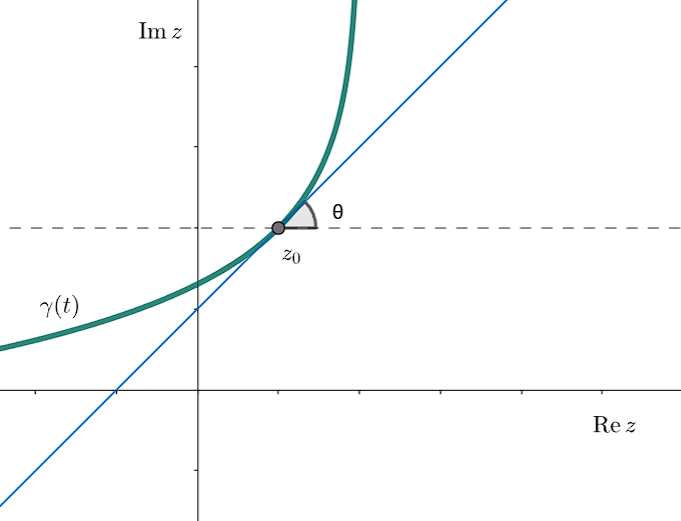
\includegraphics[height=5cm]{addchapters2/images/addchapters2_2025_03_21_1}

        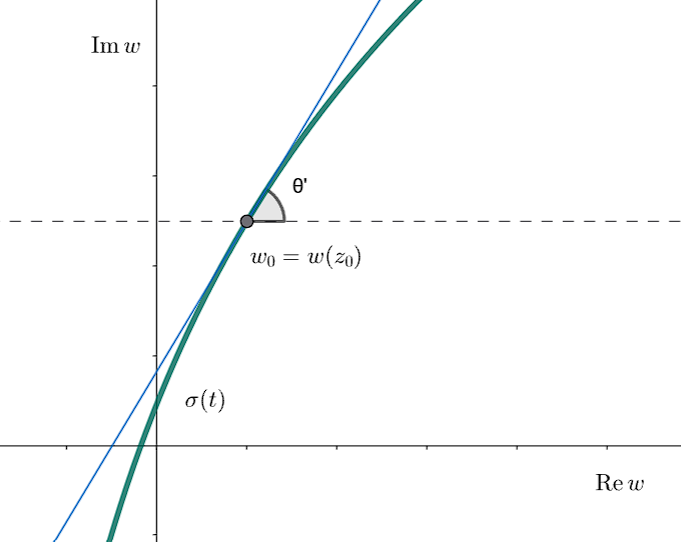
\includegraphics[height=5cm]{addchapters2/images/addchapters2_2025_03_21_2}
    \end{center}
\end{multicols}

\mediumvspace

\underline{Модуль}: $w = f(z)$ -- дифференцируема $\Longleftrightarrow \Delta w = f^\prime(z_0) \Delta z + o(\Delta z)$

Рассмотрим $\lim_{\Delta z \to 0} \left|\frac{\Delta w}{\Delta z}\right| = |f^\prime(z_0)| \Longrightarrow |\Delta w| = |f^\prime(z_0)| \cdot |\Delta z| + o(|\Delta z|)$

Рассмотрим малый контур $|\Delta z| = |z - z_0| = \rho$. Тогда $|\Delta w| = |w(z) - w(z_0)| = |f^\prime(z)| \rho + o(\rho)$

Таким образом $w(z)$ растягивает круг $|z - z_0| = \rho$ в $|f^\prime(z_0)|$ раз с точностью до малых высших порядков

\mediumvspace

\hypertarget{geometrical_meaning_of_derivative}{}

Итак, $w = f(z)$ в точке $z_0$ поворачивает точку у окрестности на угол $\alpha = \arg f^\prime(z_0)$ и растягивает отрезки $[z_0, z]$ в $k = |f^\prime(z_0)|$ раз

\hypertarget{conformal_map}{}

\Def Конформное отображение -- отображение $w(z)$, сохраняющее углы (между образами и прообразами) и постоянство растяжений

\begin{MyTheorem}
    \Ths Условия конформности: \begin{cases}\text{дифференцируемость} \\ \text{однолистность} \\ f^\prime(z) \neq 0 \text{ в } D\end{cases} $\Longleftrightarrow$ конформно
\end{MyTheorem}

\Ex $w = az + b$

\Mems Геометрический смысл линейного отображения: $b$ - перенос $z = 0$ в точку $z = b$; $a = |a| e^{i\varphi}$, тогда 
$|a|$ - коэффициент растяжения, $\varphi$ - угол поворота

Заметим, $w^\prime = (az + b)^\prime = a$, тогда $k = |w^\prime(z_0)| = |a|$, $\varphi = \arg w^\prime(z_0) = \arg a$

\Lab Проверить, что $w = z^2$ не конформное отображение, найдя $w^\prime(z_0)$

\section{3. Интеграл по комплексной переменной}

\subsection{3.1. Определения}

\smallvspace

\hypertarget{complex_integral}{}

В $\Complex$ задана кусочно-гладкая кривая $K$ (с концами в точках $M$ и $N$) параметрическими уравнениями: 

\begin{cases}
    x = \varphi(t) & \qquad t \in [\alpha, \beta] \subset \Real \\
    y = \psi(t) & \qquad \varphi, \psi \text{ -- } \Real \text{-функции} \\
\end{cases}

Тогда $z(t) = \varphi(t) + i \psi(t)$ - задание $K$ в $\Complex$. Введем отображение $w = f(z)$, действующее на $K$

Определим интегральные суммы:

\begin{enumerate}
    \item Дробление отрезка $MN$ на частичные дуги: $M = z_0, z_1, \dots, z_{n - 1}, z_n = N$

    Тогда $\alpha = t_0, t_1, \dots, t_{n - 1}, t_n = \beta$

    \item Выбор средних точек в отрезках кривой $\zeta_i = (\xi_i, \eta_i)$

    \item Сопоставим интегральную сумму $\sigma_n = \sum_{i = 1}^n f(\zeta_i) \Delta z_i$

    \item Интегралом от $w = f(z)$ по кривой $K$ называется $\lim_{\substack{n \to \infty \\ \tau = \max \Delta z_i \to 0}} \sigma_n = 
    \int_K f(z) dz$, если он существует, конечен и не зависит от способа разбиения, выбора средних точек и т. д.
\end{enumerate}

При этом интеграл можно представить как $\lim_{n \to \infty} \sigma_n = \lim_{n \to \infty} \sum_{i = 1}^n f(\zeta_i) \Delta z_i = 
\lim_{n \to \infty} \sum_{i = 1}^n f(\xi_i, \eta_i) (\Delta x_i + i \Delta y_i) = 
\lim_{n \to \infty} \sum_{i = 1}^n (u(\xi_i, \eta_i) + i v(\xi_i, \eta_i)) (\Delta x_i + i \Delta y_i) = 
\lim_{n \to \infty} \sum_{i = 1}^n (u_i \Delta x_i - v_i \Delta y_i) + i \lim_{n \to \infty} \sum_{i = 1}^n (u_i \Delta y_i + v_i \Delta x_i) =
\int_K udx - vdy + i \int_K udy + vdx$

\Nota Мы свели $\Complex$-интеграл к двум криволинейным $\Real$-интегралам, все свойства интегралов сохраняются

\Ex $\int_{\gamma = [0; 1 + i]} \overline{z} dz = \int_\gamma (x - iy) (dx + idy) = 
\int_\gamma xdx + ydy + i \int_\gamma xdy - ydx = 2 \int_0^1 xdx = 1$

% end addchapters2_2025_03_21.tex

% begin addchapters2_2025_04_04.tex





Свойства комплексного интеграла:

\begin{enumerate}[label*=\arabic*$^\circ$ ]
    \item Линейность
    \item Аддитивность
    \item Смена знака: $\int_{K^+} = - \int_{K^-}$
    \item Оценка, модуль: $\left|\int_K\right| \leq \int_K |f(z)| dz$
    \item $\int_K f(z) dz \overset{z = g(w)}{=} \int_C f(g(w)) g^\prime (w) dw = \left[\text{В частности переход к параметру } t\right] = 
    \int_{C(t)} f(t) g^\prime(t) dt$
\end{enumerate}

\Ex $I = \int_{K : |z - z_0| = \rho} \frac{dz}{z - z_0} \overset{z - z_0 = \rho e^{i\varphi}}{=} \int_K \frac{d\rho e^{i\varphi}}{\rho e^i\varphi} = 
\int_K \frac{i e^{i\varphi} d\varphi}{e^i\varphi} = i \int_0^{2\pi} d\varphi = 2\pi i$

Интеграл $I$ не зависит от радиуса и центра окружности (то есть контура интегрирования), то есть
интеграл функции $\frac{1}{z - z_0}$ будет равен $2\pi i$ для любой окружности в качестве контура 

\subsection{3.2. Теорема Коши}

\hypertarget{cauchy_for_simply_connected_space}{}

\begin{MyTheorem}
    \ThNs{1} $f(z)$ аналитическая и однозначная в односвязной области $D$

    Если $f(z)$ непрерывна на $\Gamma_D$, то $\oint_{\Gamma_D} f(z) dz = 0$
\end{MyTheorem}

\begin{MyProof}
    \begin{center}
        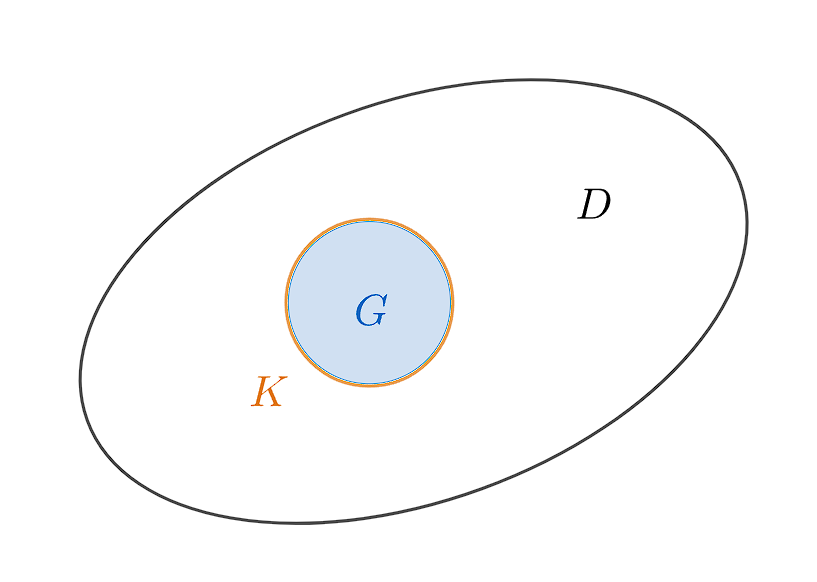
\includegraphics[width=8cm]{addchapters2/images/addchapters2_2025_04_04_1}
    \end{center}

    Запишем интеграл по контуру $K \subset D$ ($K$ - кусочно гладкая):

    $\int_K f(z) dz = \int_K u dx - vdy + i \int_K u dy + v dx = I_1 + I_2 i$

    $I_1 = \int_K \underset{P(x, y)}{\underbrace{u(x, y)}} dx - \underset{Q(x, y)}{\underbrace{v(x, y)}} dy = 
    \begin{bmatrix}f(z)\text{ - аналитическая} \Longrightarrow \\ u_x, u_y, v_x, v_y \text{ существуют} \\ \text{и непрерывны}\end{bmatrix} = 
    \underset{\text{Формула Грина}}{\iint_G \left(\frac{\partial Q}{\partial x} - \frac{\partial P}{\partial y}\right) dxdy} = 
    \iint_G \left(-\frac{\partial v}{\partial x} - \frac{\partial u}{\partial y}\right) dxdy = 
    \iint_G \left(\frac{\partial u}{\partial y} - \frac{\partial u}{\partial y}\right) dxdy = 0$

    Аналогично $I_2 = \int_k udy + vdx = \iint_G \left(\frac{\partial u}{\partial x} - \frac{\partial v}{\partial y}\right) dxdy = 
    \iint_G \left(\frac{\partial u}{\partial x} - \frac{\partial u}{\partial x}\right) dxdy = 0$

    Таким образом, $\oint_{K \subset D} f(z) dz = 0$ - формула Коши

    Так как $f(z)$ непрерывна на $\Gamma_D$, то можно взять $K = \Gamma_D$
\end{MyProof}

\Nota Получим, что интеграл по любому замкнутому $\Gamma_D$ контуру в области аналитичности равен нулю

То есть $\int_{AB} f(z) dz$ в условиях \ThNs{1} не зависит от пути, и его можно решать как $\int_{AB} = \int_A^B$

\Nota Обобщим \ThNs{1} на многосвязную область. Выколотые области тоже имеют границы, которые включены в границу всей области

\hypertarget{cauchy_for_connected_space}{}

\begin{MyTheorem}
    % https://www.geogebra.org/calculator/ujuysjcp
    
    \begin{center}
        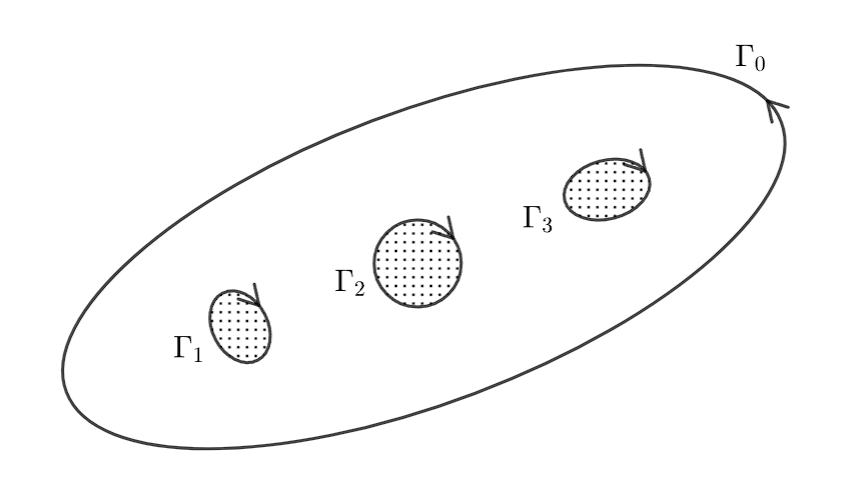
\includegraphics[width=10cm]{addchapters2/images/addchapters2_2025_04_04_2}
    \end{center}
    
    \ThNs{2} Дана многосвязная область $D$, $f(z)$ - аналитична в $D$ и непрерывна на $\Gamma_D$


    Граница $\Gamma_D = \Gamma_0 \cup \Gamma_1 \cup \Gamma_2 \cup \dots \cup \Gamma_n$, где положительным обходом области
    считается тот, при котором область обхода слева

    Тогда $\int_{\Gamma_D^+} f(z) dz = 0$ или $\int_{\Gamma_0 \CounterClockwiseArrow} f(z) dz = \sum_{i = 1}^n \int_{\Gamma_i \CounterClockwiseArrow} f(z) dz$ 
\end{MyTheorem}


\begin{MyProof}
    Сделаем разрезы как на картинке. 
    Разрезы превратили область $D$ в односвязную с границей $\Gamma^\prime = \Gamma_0 \cup (\gamma_1^+ \cup \gamma_1^- \cup \Gamma_1) \cup \dots = \Gamma_0 \cup \bigcup_{i = 1}^n (\gamma_i^+ \cup \gamma_i^- \cup \Gamma_i)$

    \begin{center}
        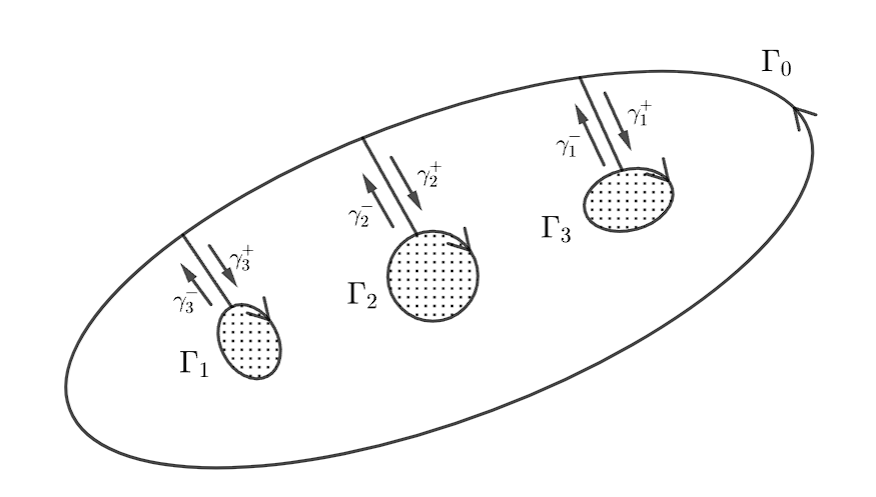
\includegraphics[width=10cm]{addchapters2/images/addchapters2_2025_04_04_3}
    \end{center}

    По \ThNs{1} $\int_{\Gamma^\prime} f(z) dz = 0 \Longleftrightarrow \int_{\Gamma_D} f(z) dz + \int_{\gamma^+_1} f(z) dz + \int_{\gamma^-_1} f(z) dz + \int_{\Gamma_1} f(z) dz + \dots = 0$

    Но $\int_{\gamma_1^+} = - \int_{\gamma_1^-}$, поэтому $\int_{\Gamma_D^+} = \sum \int_{\Gamma_i^-}$ или $\int_{\Gamma_0 \CounterClockwiseArrow} = \sum \int_{\Gamma_i \CounterClockwiseArrow}$
\end{MyProof}

% https://www.geogebra.org/calculator/rdsykgz5

\begin{wrapfigure}{R}{0pt}
    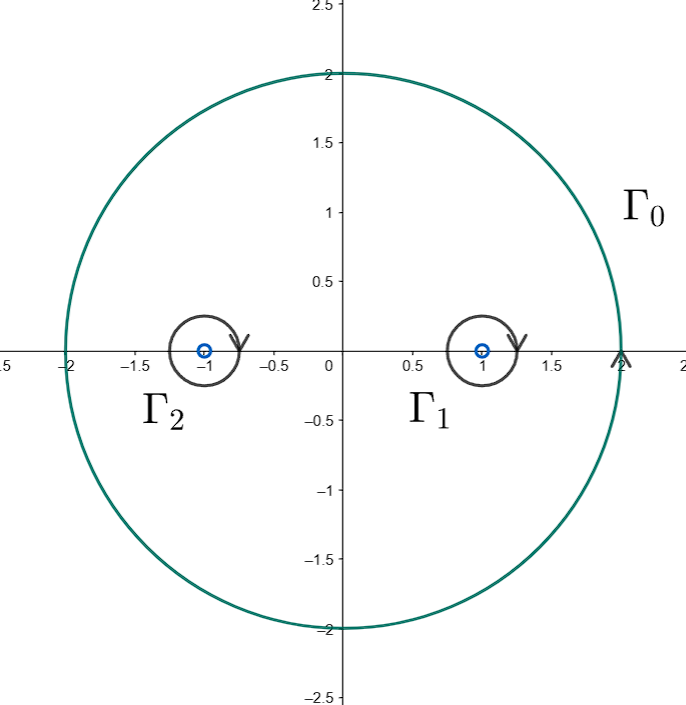
\includegraphics[width=4.5cm]{addchapters2/images/addchapters2_2025_04_04_4}
\end{wrapfigure}

\Ex $\int_{|z| = 2} f(z) dz$

По \ThNs{2} $\int_{\Gamma_0 \CounterClockwiseArrow} f(z) dz + \int_{\Gamma_1 \ClockwiseArrow} f(z) dz + \int_{\Gamma_2 \ClockwiseArrow} f(z) dz = 0$

Тогда $\int_{|z| = 2 \CounterClockwiseArrow} f(z) dz = \int_{|z - 1| = \rho_1 \CounterClockwiseArrow} f(z) dz + \int_{|z + 1| = \rho_2 \CounterClockwiseArrow} f(z) dz$,
где $\rho_1$, $\rho_2$ - радиусы бесконечно малой длины 

\subsection{3.3. Неопределенный интеграл}

\hypertarget{antiderivative}{}

\Mem По теореме Барроу $\Phi(x) = \int_{x_0}^x f(t) dt$ - интеграл с переменным верхним пределом

Тогда $\Phi(x)$ - дифференцируема, и $\Phi^\prime(x) = f(x)$, то есть $\Phi(x)$ - первообразная $f(x)$

\begin{MyTheorem}
    \Ths $f(z)$ непрерывна в односвязной области $D$ и $\forall \Gamma \subset D \ \int_\Gamma f(z) dz = 0$

    Тогда при фиксированном $z_0 \in D \ \Phi(z) = \int_{z_0}^z f(\zeta) d\zeta$ аналитична в $D$ и $\Phi^\prime(z) = f(z)$
\end{MyTheorem}

\begin{MyProof}
    Если $\forall \Gamma \ \int_\Gamma f(z) dz = 0$, то $\Phi(z) = \int_{z_0}^z F(\zeta) d\zeta$ - интеграл, не зависящий от пути, а только от $z_0$ и $z$

    Рассмотрим $\frac{\Phi(z + \Delta z) - \Phi(z)}{\Delta z} = \frac{1}{\Delta z} \left(\int_{z_0}^{z + \Delta z} f(\zeta) d\zeta - \int_{z_0}^z f(\zeta) d\zeta\right) = 
    \frac{1}{\Delta z} \int_z^{z + \Delta z} f(\zeta) d\zeta = \frac{1}{\Delta z} \int_z^{z + \Delta z} (f(\zeta) - f(z) + f(z))d\zeta = 
    \frac{1}{\Delta z} \int_z^{z + \Delta z} f(z) d\zeta + \frac{1}{\Delta z} \int_z^{z + \Delta z} (f(\zeta) - f(z))d\zeta = 
    \cancelto\frac{1}{\Delta z}  f(z) \cancelto{\zeta \Big|_{z}^{z + \Delta z}} + \frac{1}{\Delta z} \int_z^{z + \Delta z} (f(\zeta) - f(z))d\zeta$

    $\left|\int_z^{z + \Delta z} (f(\zeta) - f(z)) d\zeta\right| \leq \int_z^{z + \Delta z} |f(\zeta) - f(z)| d\zeta \leq \max_{[z, z + \Delta z]} |f(\zeta) - f(z)| \Delta z$

    Так как $f(z)$ непрерывна в $D$ и $z, \zeta \in D$, то $\lim_{\zeta \to z} f(\zeta) = f(z) \Longleftrightarrow 
    \forall \varepsilon > 0 \ \exists \delta > 0 \ | \ 0 < |\zeta - z| < \delta \ |f(\zeta) - f(z)| < \varepsilon$

    Тогда $\forall \varepsilon > 0 \ \exists \delta > 0 \ | \ 0 < |\zeta - z| < \delta \ \max |f(\zeta) - f(z)| < \varepsilon$

    То есть $\left|\int_z^{z + \Delta z} (f(\zeta) - f(z)) d\zeta \right| \leq \varepsilon \Delta z$

    Или $\frac{\Phi(z + \Delta z) - \Phi(z)}{\Delta z} \leq f(z) + \varepsilon$, то есть $\left|\frac{\Delta \Phi}{\Delta z} - f(z)\right| < \varepsilon$,
    или $\lim_{\Delta z \to 0} \frac{\Phi(z + \Delta z) - \Phi(z)}{\Delta z} = \Phi^\prime(z) = f(z)$
\end{MyProof}

\Def $\Phi(z) = \int_{z_0}^z f(\zeta) d\zeta$ называют первообразной для $f(z)$

Следствие - формула Ньютона-Лейбница: \fbox{$\int_{z_1}^{z_2} f(\zeta) d\zeta = \Phi(z_2) - \Phi(z_1)$}

\subsection{3.4. Интеграл Коши}

% https://www.geogebra.org/calculator/vzfpbwz9

\begin{wrapfigure}{R}{0pt}
    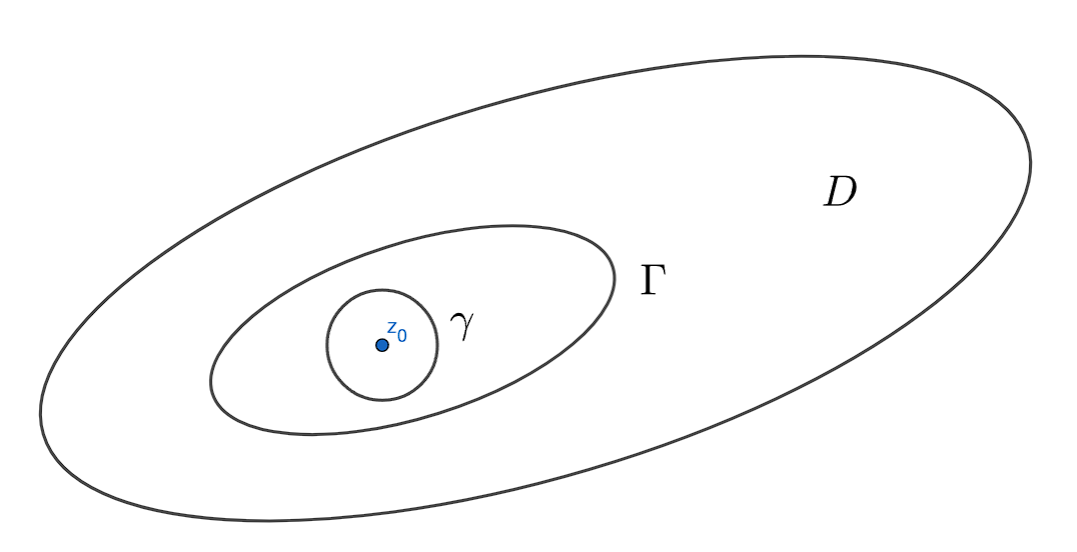
\includegraphics[width=7cm]{addchapters2/images/addchapters2_2025_04_04_5}
\end{wrapfigure}


\Nota Установим связь между значениями $f(z)$ во внутренних точках области и на ее границе

$f(z)$ аналитична в односвязной области $D$, $z_0 \in D$. Окружаем $z_0$ контуром $\Gamma \in D$ и меньшим контуром
$\gamma: |z - z_0| = \rho$

В кольце между $\gamma$ и $\Gamma$ рассмотрим функцию $\varphi(z) = \frac{f(z)}{z - z_0}$ (в кольце $\varphi(z)$ аналитична)

По \ThNs{2} для $\varphi(z)$ в многосвязной области $\int_{\Gamma \CounterClockwiseArrow} \varphi(\zeta) d\zeta = \int_{\gamma \CounterClockwiseArrow} \varphi(\zeta) d\zeta$ - не зависит от пути 

То есть выбор окружности в качестве $\gamma$ не важен:

$\int_{\gamma \CounterClockwiseArrow} \varphi(\zeta) d\zeta \overset{z - z_0 = \rho e^{i\varphi}}{=} \int_0^{2\pi} \frac{f(\zeta) \rho i e^{i\varphi} d\varphi}{\rho e^{i \varphi}} = i \int_0^{2\pi} f(\zeta) d\varphi = 
\underset{\text{стягиваем } \gamma \text{ в точку } z_0, \int \to 0}{\underbrace{i \int_0^{2\pi} (f(\zeta) - f(z_0)) d\varphi}} + i \int_0^{2\pi} f(z_0) d\varphi = i f(z_0) \cdot 2\pi$

Тогда $\int_\Gamma \frac{f(z)}{z - z_0} dz = \int_\gamma \varphi(\zeta) d\zeta = 2\pi i f(z_0)$

\Nota Доказали теорему: в области аналитичности $\forall z_0 \in D \ \int_{\Gamma_D} \frac{f(z)}{z - z_0} dz = 2 \pi i f(z_0)$

\Ex $\int_{|z| = 2 \CounterClockwiseArrow} \frac{f(z)}{(z - 1)(z + 1)} dz = \int_{|z - 1| = \rho_1 \CounterClockwiseArrow} \frac{\frac{f(z)}{z + 1}}{z - 1} dz + \int_{|z + 1| = \rho_2 \CounterClockwiseArrow} \frac{\frac{f(z)}{z - 1}}{z + 1} dz = 
2\pi i \left(\frac{f(1)}{2} + \frac{f(-1)}{-2}\right)$

% end addchapters2_2025_04_04.tex

% begin addchapters2_2025_04_18.tex






\section{4. Ряды}

\subsection{4.1. Числовой ряд в комплексной плоскости}

\hypertarget{complex_series}{}

\DefN{1} $z_1 + z_2 + \dots + z_n + \dots = \sum_{n = 1}^\infty z_n$, где $z_n \in \Complex$ - числовой ряд

\DefNs{2} Сумма ряда - $S = \lim_{n \to \infty} S_n = \lim_{n \to \infty} \sum_{k = 1}^n z_k$

Если сумма существует и конечна, то ряд называют сходящимся. 

\Def $f(z)$ называется регулярной в точке $z_0$, если $f(z_0) = \sum_{n = 1}^\infty c_n$, где $c_n \in \Complex$

\Nota Для комплексных числовых рядов остаются справедливыми:

\begin{enumerate}
    \item Необходимое условие сходимости
    \item Признак Даламбера
    \item Радикальный признак Коши
    \item Критерий Коши
    \item Абсолютная сходимость
\end{enumerate}

\subsection{4.2. Функциональный ряд в комплексной плоскости}

\Def $\sum_{n = 1}^\infty u_n(z)$, где $u_n(z) : \ D \subset \Complex \longrightarrow \Complex$ - функциональный ряд

\begin{MyTheorem}
    \ThNs{Признак Вейерштрасса}

    $\exists \sum_{n = 1}^\infty \alpha_n$, $\alpha_n \in \Real_0^+$, $\sum_{n = 1}^\infty \alpha_n \in \Real$,
    $|u_n(z)| \leq \alpha_n \ \forall z \in D \Longrightarrow \sum_{n = 1}^\infty u_n(z)$ сходится равномерно в $D$
\end{MyTheorem}

\Lab Сверить формулировку и доказательства для $\Complex$ и $\Real$-случая 

\Nota Сумма равномерно сходящегося ряда непрерывна

\begin{MyTheorem}
    \Ths $u_n(z)$ непрерывна в $D$ и $f(z) = \sum_{n = 1}^\infty u_n(z)$ сходится равномерно в $D$

    Тогда $\int_K f(\zeta) d\zeta = \sum_{n = 1}^\infty \int_K u_n(\zeta) d\zeta$, где $K \subset D$ - кусочно гладкая кривая
\end{MyTheorem}

\begin{MyProof}
    Докажем, что $\left|\int_K f(\zeta) d\zeta - \sum_{k = 1}^n \int_K u_k(\zeta) d\zeta\right| \underset{n \to \infty}{\longrightarrow} 0$

    $\left|\int_K \left(f(\zeta) - \sum_{k = 1}^n u_k(\zeta)\right) d\zeta\right| =
    \left|\int_K \left(\sum_{k = 1}^\infty u_k(\zeta) - \sum_{k = 1}^n u_k(\zeta)\right) d\zeta\right| = 
    \left|\int_K \sum_{k = n + 1}^\infty u_k(\zeta) d\zeta\right| = \left|\int_K r_n(\zeta) d\zeta \right| \leq
    \int_K |r_n(\zeta)| |d\zeta| \underset{\text{по кр. Коши}}{\leq \varepsilon}$
\end{MyProof}


\subsection{4.3. Степенной ряд}

\hypertarget{complex_power_series}{}

\Def Степенной ряд - $\sum_{n = 0}^\infty c_n (z - a)^n \qquad \left(a = 0: \sum_{n = 0}^\infty c_n z^n\right)$, $c_n \in \Complex$

\Nota Область сходимости - круг с центром $a$, $|z - a| \leq R$ - радиус сходимости 

$\lim_{n \to \infty} \left|\frac{c_{n + 1} (z - a)^{n + 1}}{c_n (z - a)^n}\right| = \lim_{n \to \infty} \left|\frac{c_{n + 1}}{c_n}\right| |z - a| < 1 \Longrightarrow |z - a| < \left|\frac{c_n}{c_{n + 1}}\right|$

\Nota Также справедлива теорема Абеля

\hypertarget{abels_theorem}{}

\begin{MyTheorem}
    \ThNs{Абеля} 
    
    Если степенной ряд сходится в точке $z_1$, то он сходится абсолютно и равномерно 
    в любой точке $z_2$ такой, что $|z - z_1| > |z - z_2|$

    Если степенной ряд расходится в точке $z_1$, то он расходится
    в любой точке $z_2$ такой, что $|z - z_1| < |z - z_2|$
\end{MyTheorem}


Следствие: Если $f(z) = \sum_{n = 0}^\infty c_n z^n$, то $f(z)$ - непрерывна в круге сходимости ряда

\begin{MyTheorem}
    \ThNs{Почленное дифференцирование суммы ряда}

    $\sum_{n = 0}^\infty c_n z^n = f(z)$ - сходящийся в круге радиуса $R \neq 0$. Тогда $f(z)$ дифференцируема и 
    $f^\prime(z) = \sum_{n = 0}^\infty n c_n z^{n - 1}$
\end{MyTheorem}

\begin{MyProof}
    Рассмотрим ряд (и его сумму) $\sum_{n = 0}^\infty n c_n z^{n - 1}$ - он сходится в круге радиуса $\rho$ таком, что $0 \leq |z| \leq \rho < R$
    (см. сходимость по Даламберу) (Обозначим круг $K_1 : |z| = \rho$)

    Докажем, что $\sum_{n = 0}^\infty n c_n z^{n - 1} = S(z) = f^\prime(z)$

    В круге $K_1$ выберем кривую $\gamma$, соединяющую $z_0 = 0$ и $z$

    Рассмотрим $\int_\gamma \zeta^k d \zeta$, функция $\zeta^k$ аналитическая, тогда $\int_\gamma \zeta^k d\zeta$ не зависит от пути 

    $\int_\gamma \zeta^k d\zeta = \int_0^z \zeta^k d\zeta = \frac{\zeta^{k + 1}}{k + 1} \Big|^z_0 = \frac{z^{k + 1}}{k + 1}$

    Тогда $\int_0^z n c_n \zeta^{n - 1} d\zeta = \frac{n c_n \zeta^n}{n} \Big|_0^z = c_n z^n$

    Возьмем интеграл от суммы $\int_0^z S(\zeta) d\zeta = \int_0^z \left(\sum_{n = 0}^\infty n c_n \zeta^{n - 1}\right) d\zeta = 
    \sum_{n = 0}^\infty \int_0^z n c_n \zeta^{n - 1} d\zeta = \sum_{n = 0}^\infty c_n z^n = f(z)$

    Таким образом, $f(z)$ является первообразной для $S(z)$, то есть $S(z) = f^\prime(z)$

    При этом $f^\prime (z) = \sum_{n = 0}^\infty n c_n z^{n - 1} = \sum_{m}^\infty c_m z^m$ - этот ряд
    можно дифференцировать дальше, и область, в которой функция дифференцируется, - круг $K_1$, где $\rho$ вплотную подходит к $R$

    Таким образом, доказали, что если $f(z)$ регулярна $\forall z$ в круге $|z| < R$, то $f(z)$ сколько угодно раз дифференцируема в этом круге и $f^\prime(z) = \left(\sum_{n = 0}^\infty c_n z^n\right)^\prime$
\end{MyProof}

Следствие: $f^\prime(z) = (c_0 + c_1 z + c_2 z^2 + \dots + c_n z^n + \dots)^\prime$ или 
$f^\prime(z) = (c_0 + c_1 (z - a) + c_2 (z - a)^2 + \dots + c_n (z - a)^n + \dots)^\prime \Longrightarrow c_0 = f(a), c_1 = f^\prime(a), c_2 = \frac{f^\prime^\prime(z)}{2!}$ и так далее 

Получили ряд Тейлора $f(z) \underset{|z - a| < \rho}{=} \sum_{n = 0}^\infty \frac{f^{(n)} (a)}{n!} (z - a)^n$

\begin{MyTheorem}
    \Ths $f(z)$ аналитическая в области $D$ $\Longrightarrow f(z)$ регулярна в области $D$
\end{MyTheorem}

\begin{MyProof}
    По формуле Коши $f(z) = \frac{1}{2\pi i} \int_{\gamma_\rho} \frac{f(\zeta)}{\zeta - z} d\zeta \ \forall z \in K$, где $K = \{z \ | \ |z - a| < \rho\}$, $\gamma_\rho = \{ \zeta \ | \ |\zeta - a| = \rho\}$ и $K \subset D$

    Разложим в ряд $\frac{1}{\zeta - z}$:

    $\frac{1}{\zeta - z} = \frac{1}{\zeta - (z - a) - a} = \frac{1}{\zeta - a} \cdot \frac{1}{1 - \frac{z - a}{\zeta - a}} = \frac{1}{\zeta - a} \sum_{n = 0}^\infty \left(\frac{z - a}{\zeta - a}\right)^n$, где $\left|\frac{z - a}{\zeta - a}\right| < 1$

    То есть $\sum_{n = 0}^\infty \frac{(z - a)^n}{(\zeta - a)^{n + 1}}$ - равномерно сходящийся

    Тогда $\frac{f(\zeta)}{\zeta - z} = \sum_{n = 0}^\infty \frac{f(\zeta) (z - a)^n}{(\zeta - a)^{n + 1}}$ - равномерно сходящийся 

    $\frac{1}{2\pi i} \int_{\gamma_\rho} \frac{f(\zeta)}{\zeta - z} = \frac{1}{2\pi i} \sum_{n = 0}^\infty \left(\int_{\gamma_\rho} \frac{f(\zeta)}{(\zeta - a)^{n + 1}} d\zeta \right) (z - a)^n$

    $f(z) = \sum_{n = 0}^\infty b_n (z - a)^n$ - единственное разложение по Тейлору, где $b_n = \int_{\gamma_\rho} \frac{f(\zeta)}{(\zeta - a)^{n + 1}} d\zeta$

    Итак $\frac{1}{2\pi i} \int_{\gamma_\rho} \frac{f(\zeta) d\zeta}{(\zeta - a)^{n + 1}} = \frac{f^{(n)}(a)}{n!}$
\end{MyProof}

% end addchapters2_2025_04_18.tex

% begin addchapters2_2025_05_02.tex





\begin{MyTheorem}
    \ThNs{Морера} $f(z)$ непрерывна в $D$ и $\forall \gamma \subset D \ \int_\gamma f(z) dz = 0 \Longrightarrow f(z)$ аналитична в $D$
\end{MyTheorem}

\begin{MyProof}
    При данных условиях $\exists \Phi(z) = \int_{z_0}^z f(\zeta) d\zeta \ | \ \Phi^\prime(z) = f(z)$ и $\Phi(z)$ аналитична

    Так как $\Phi(z)$ дифференцируема, то она дифференцируема сколько угодно раз. Таким образом, существуют $f^\prime(z), f^{\prime\prime}(z)$ и так далее, а из этого означает, что $f(z)$ -- аналитична
\end{MyProof}


\begin{MyTheorem}
    \ThNs{Лиувилля} $f(z)$ аналитична в $\Complex$ и $\exists M \in \Real^+ \ | \ |f(z)| \leq M \ \forall z \in \Complex$

    Тогда $f(z) \equiv \const$
\end{MyTheorem}


\begin{MyProof}
    Докажем, что $f^\prime(z) = 0$

    $|f^\prime(z)| = \begin{bmatrix}\text{контур } \gamma \text{ -- круг } z + \rho e^{i\varphi} \end{bmatrix} = \left|\frac{1}{2\pi i} \int_\gamma \frac{f(\zeta)}{(\zeta - z)^2} d\zeta\right| = \left|\frac{1}{2\pi i}\int_0^{2\pi} \frac{f(z + \rho e^{i \varphi}) \rho i e^{i \varphi}}{\rho ^2 e^{2 i \varphi}} d\varphi \right| \leq \frac{1}{2\pi} \int_0^{2\pi} \left| \frac{f(z + \rho e^{i \varphi})}{\rho e^{i \varphi}}\right| d\varphi \leq \frac{1}{2\pi} \int_0^{2\pi} \frac{M}{\rho} d\varphi = \frac{M}{\rho} \underset{\rho \to \infty}{\longrightarrow} 0 \Longrightarrow f(z) = \const$
    
\end{MyProof}

\Nota $w = \sin z \neq \const \Longrightarrow \sin z$ -- неограниченная функция

\subsection{4.4. Ряд Лорана}

\hypertarget{laurent_series}{}

\Def Ряд вида $\sum_{n = -\infty}^\infty C_n (z - z_0)^n$, где $C_n, z_0 \in \Complex$, называется рядом Лорана в точке $z_0$

% https://www.geogebra.org/calculator/mxctddsq

\begin{wrapfigure}[6]{R}{0pt}
    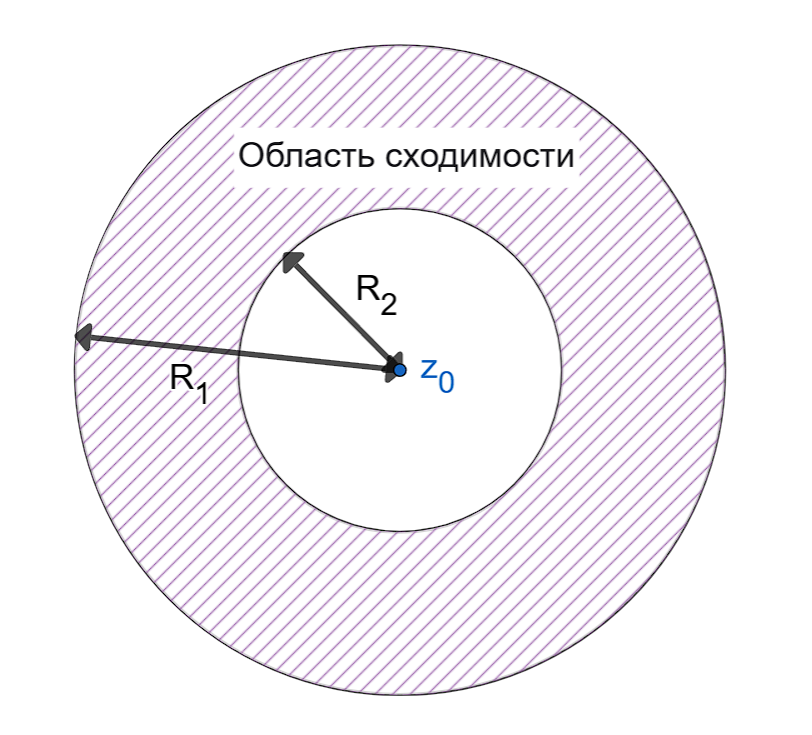
\includegraphics[width=6cm]{addchapters2/images/addchapters2_2025_05_02_1}
\end{wrapfigure}

\Nota Исследуем ряд. Обозначим $f_1 = \sum_{n = 0}^\infty C_n (z - z_0)^n$

$f_2 = \sum_{n = -1}^{-\infty} C_n (z - z_0)^n \overset{m = -n}{\Longrightarrow} \sum_{m = 1}^\infty \frac{C_{-m}}{(z - z_0)^m} = \sum_{n = 1}^\infty \frac{C_{-n}}{(z - z_0)^n}$

Тогда ряд можно записать так: $C_0 + \sum_{n = 1}^\infty \left(C_n (z - z_0)^n + \frac{C_{-n}}{(z - z_0)^n}\right)$

Рассмотрим $f_1 = \sum_{n = 0}^\infty C_n (z - z_0)^n$ -- ряд согласно теореме Абеля сходится в круге с центром $z_0$ и радиусом $R_1 = \lim_{n \to \infty} \left|\frac{C_{n}}{C_{n+1}}\right|$

Рассмотрим $f_2 = \sum_{n = 1}^\infty \frac{C_{-n}}{(z - z_0)^n} \overset{t = \frac{1}{z - z_0}}{=\joinrel=\joinrel=} \sum_{n = 1}^\infty C_{-n} t^n$ -- ряд сходится в круге $|t| < r = \lim_{n \to \infty} \left|\frac{C_{-n}}{C_{-n-1}}\right|$ или $|z - z_0| > \lim_{n \to \infty} \left|\frac{C_{-n-1}}{C_{-n}}\right| = R_2$

Таким образом, ряд Лорана сходится в \textit{кольце} с внутренним радиусом $R_2$ и внешним радиусом $R_1$ и центром $z_0$ к значению некой аналитической функции $f(z)$


\begin{MyTheorem}
    $f(z)$, аналитичная в кольце $K = (z_0, R_2, R_1)$, однозначно представима рядом Лорана в кольце $K$
\end{MyTheorem}

\begin{MyProof}
    \begin{wrapfigure}[6]{R}{5.2cm}
        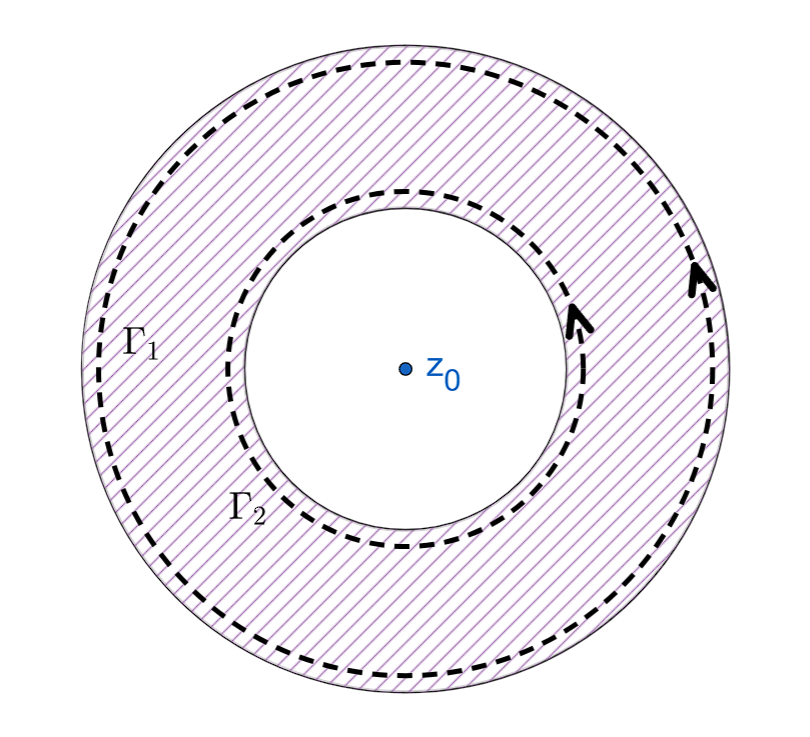
\includegraphics[width=\linewidth]{addchapters2/images/addchapters2_2025_05_02_2}
    \end{wrapfigure}

    $f(z) = \frac{1}{2\pi i} \int_\Gamma \frac{f(\zeta)}{\zeta - z} d\zeta \overset{\Gamma = \Gamma_2 \cup \Gamma_1}{=\joinrel=\joinrel=\joinrel} \frac{1}{2\pi i} \int_{\Gamma_1} \frac{f(\zeta)}{\zeta - z}d\zeta - \frac{1}{2\pi i} \int_{\Gamma_2} \frac{f(\zeta)}{\zeta - z} d\zeta$

    Разложим $\frac{1}{\zeta - z}$ в ряд Тейлора:

    $\frac{1}{\zeta - z} = \frac{1}{\zeta - z_0 - (z - z_0)} = 
    \begin{sqcases}
        \frac{1}{(\zeta - z_0)(1 - (\frac{z - z_0}{\zeta - z_0}))} = \sum_{n = 1}^\infty \frac{(z - z_0)^n}{(\zeta - z_0)^{n + 1}}\\ 
        \frac{1}{-(z - z_0)(1 - (\frac{\zeta - z_0}{z - z_0}))} = -\sum_{n = 1}^\infty \frac{(\zeta - z_0)^n}{(z - z_0)^{n + 1}}
    \end{sqcases}$

    1. Первый ряд сходится, если $\frac{z - z_0}{\zeta - z_0} < 1 \Longleftrightarrow |z - z_0| < |\zeta - z_0|$ -- это $\Gamma_1$

    Также $\frac{f(\zeta)}{\zeta - z} = \sum_{n = 0}^\infty \frac{f(\zeta)(z - z_0)^n}{(\zeta - z_0)^{n + 1}}$

    По теореме Коши:

    $f(z) = \frac{1}{2\pi i} \int_{\Gamma_1} \frac{f(\zeta)}{\zeta - z} d\zeta = \frac{1}{2\pi i} \sum_{n = 0}^\infty \left(\int_{\Gamma_1} \frac{f(\zeta)d\zeta}{(\zeta - z_0)^{n + 1}}\right) (z - z_0)^n = \sum_{n = 0}^\infty C_n (z - z_0)^n$

    Из этого $C_n = \frac{1}{2\pi i} \int_{\Gamma_1} \frac{f(\zeta)d\zeta}{(\zeta - z_0)^{n + 1}}$ \\

    2. Второй ряд сходится, если $\frac{z - z_0}{\zeta - z_0} < 1 \Longleftrightarrow |z - z_0| > |\zeta - z_0|$ -- это $\Gamma_2$

    \Lab
\end{MyProof}

\Nota Таким образом, коэффициенты ряда Лорана $C_n = \frac{1}{2\pi i} \int_{\Gamma_i} \frac{f(\zeta)}{(\zeta - z_0)^{n + 1}} d\zeta$

\hypertarget{isolated_special_point}{}

\Def Изолированной особой точкой однозначного характера называется точка $a \in \Complex \ | \ f(z)$ аналитична в кольце $0 < |z - a| < \rho$, но не определена в $z = a$

\Defs Точка $a = \infty$ называется изолированной особой, если $f(z)$ аналитична в кольце $\rho < |z| < \infty$

\Defs Устранимой особой точкой $a$ называется точка, для которой $\lim_{z \to a} f(z) \in \Complex$, в $a$ функция не определена

Полюсом $a$ называется точка, для которой $\lim_{z \to a} f(z) = \infty$

Существенно особой точкой $a$ называется точка, для которой $\nexists \lim_{z \to a} f(z)$

\ExN{1} Для $f(z) = \frac{\sin z}{z}$ точка $z = 0$ является устранимой особой -- $\lim_{z \to 0} \frac{\sin z}{z} = 1$

\ExNs{2} Для $f(z) = \frac{z}{(z + i)^2} \quad \lim_{z \to -i} \frac{z}{(z + i)^2} = \left[\frac{1}{0^2} = \infty^2\right]$, $a = -i$ - полюс 2-ого порядка

\ExNs{3} Для $f(z) = \sin z \quad \nexists \lim_{z \to \infty} \sin z$ 

\Def Для ряда Лорана функции $f(z)$ в окрестности особой точки $z = a \in \Complex \quad f(z) = \underset{\text{это правильная часть}}{\underbrace{\sum_{n = 0}^\infty C_n (z - a)^n}} + \underset{\text{это главная часть}}{\underbrace{\sum_{n = 1}^\infty \frac{C_{-n}}{(z - a)^n}}}$

\Def Для ряда Лорана в $a = \infty$: $f(z) = \sum_{n = -\infty}^\infty C_n z^n = \underset{\text{это главная часть}}{\underbrace{\sum_{n = 1}^\infty C_n z^n}} + \underset{\text{это правильная часть}}{\underbrace{\sum_{n = 0}^\infty \frac{C_{-n}}{z^n}}}$

\hypertarget{residuum}{}

\Def Вычетом $\residuum(f(z), z_0)$ функции $f(z)$ в точке $z_0$ называется $C_{-1}$ коэффициент ряда Лорана, если $z_0 \in \Complex$, и $-C_{-1}$, если $z_0 = \infty$



% end addchapters2_2025_05_02.tex

% begin addchapters2_2025_05_16.tex





Из определения ясно, что для конечной точки $\residuum(f(z), z_0) = C_{-1} = \frac{1}{2\pi i} \int_\gamma \frac{f(\zeta)}{(\zeta - z_0)^0} d\zeta = \frac{1}{2\pi i} \int_\gamma f(\zeta) d\zeta$

Для бесконечной $\residuum(f(z), z_0) = -C_{-1} = -\frac{1}{2\pi i} \int_{\gamma^+} f(\zeta) d\zeta = \frac{1}{2\pi i} \int_{\gamma^-} f(\zeta) d\zeta$

Здесь вместо $\gamma$ берут для простоты окружность

\Nota Для вычисления вычетов используют более простые формулы, которые зависят от типа особых точек

\begin{MyTheorem}
    \ThNs{1} $z_0$ -- устранимая особая точка ($z_0 \in \Complex$) функции $f(z) \Longleftrightarrow$ главная часть ряда Лорана равна 0
    
    То есть $f(z)$ в $z_0$ представима как $\sum_{n = 0}^\infty C_n (z - z_0)$ тогда и только тогда, когда $\lim_{z \to z_0} f(z) \in \Complex$
\end{MyTheorem}

\begin{MyProof}
    \fbox{$\Longrightarrow$} $z_0$ -- устранимая $\Longleftrightarrow \lim_{z \to \z_0} f(z) = A \in \Complex$

    Тогда в некоторой окрестности $\overset{\circ}{U}_\delta (z_0)$ функция ограничена -- $|f(z)| \leq M, M \in \Real$

    $C_{-n} = \frac{1}{2\pi i} \int_{\gamma_\delta} \frac{f(\zeta)d\zeta}{(\zeta - z)^{-n + 1}} = \left[\gamma_\delta: \zeta = z_0 + \delta e^{i\phi}\right] = \frac{1}{2\pi i} \int_{0}^{2\pi} \frac{f(\zeta) \delta i e^{i\varphi} d\varphi}{(\delta e^{i\varphi})^{-n + 1}} = \frac{1}{2\pi} \int_0^{2\pi} f(\zeta) \delta^{n} e^{ni\varphi} d\varphi$

    $|C_{-n}| \leq \frac{1}{2\pi} \int_0^{2\pi} M \delta^n d\varphi = M \delta^n \underset{\delta \to 0}{\longrightarrow} 0$

    \mediumvspace

    \fbox{$\Longleftarrow$} $C_{-n} = 0 \Longrightarrow f(z) = \sum_{n = 0}^\infty C_n (z - z_0)^n = C_0 + C_1 (z - z_0) + \dots$

    $\lim_{z \to z_0} f(z) = C_0 \in \Complex$ -- устранимая
\end{MyProof}

\underline{Следствие}: вычет в устранимой точке равен 0

\begin{MyTheorem}
    \ThNs{2} $z_0$ -- полюс $m$-ого порядка $\Longleftrightarrow$ главная часть ряда Лорана содержит не более $m$ ненулевых членов подряд (то есть для $i > m \ C_{-i} = 0$) 
\end{MyTheorem}

\begin{MyProof}
    Полюс $m$-ого порядка функции $f(z)$ -- точка $z_0$, для которой $\lim_{z \to z_0} f(z) = \infty \Longrightarrow \lim_{z \to z_0} \frac{1}{f(z)} = \lim_{z \to z_0} g(z) = 0$ и $z_0$ -- ноль функции $g(z)$ порядка $m$
    
    То есть $g(z)$ представима как $g(z) = (z - z_0)^m h(z)$, где $h(z)$ -- аналитическая в $z_0$ и $h(z_0) \neq 0$

    \fbox{$\Longrightarrow$} Рассмотрим $\frac{1}{h(z)} = \sum_{n = 0}^\infty b_n (z - z_0)^n$, при этом $\frac{1}{h(z_0)} = b_0 \neq 0$ ($h(z)$ -- аналитическая $\Longrightarrow \frac{1}{h(z)}$ -- аналитическая $\Longrightarrow \frac{1}{h(z)}$ -- регулярная)

    $f(z) = \frac{1}{g(z)} = \frac{1}{(z - z_0)^m h(z)} = \frac{1}{(z - z_0)^m} \sum_{n = 0}^\infty b_n (z - z_0)^n = \frac{1}{(z - z_0)^m} (b_0 + b_1 (z - z_0) + \dots) = \underset{\frac{C_{-m}}{(z - z_0)^m} \neq 0}{\underbrace{\frac{b_0}{(z - z_0)^m}}} + \frac{b_1}{(z - z_0)^{m - 1}} + \dots + \frac{b_n}{(z - z_0)^{m - n}} + \dots = \sum_{n = -m}^\infty C_n (z - z_0)^n$

    При этом $C_{-n} = 0$ при $n \geq m + 1$

    \mediumvspace

    \fbox{$\Longleftarrow$} $f(z) = \sum_{n = -m}^\infty C_n (z - z_0)^n = \frac{C_{-m}}{z - z_0}^m + \dots + \frac{C_{-1}}{z - z_0} + C_0 + C_1 (z - z_0) + \dots = \frac{1}{(z - z_0)^m} \underset{\text{аналитическая } \frac{1}{h(z)} \text{ в } z_0}{\underbrace{(C_{-n} + \dots + C_{-1} (z - z_0)^{m - 1} + C_0 (z - z_0)^m + \dots)}} = \frac{1}{(z - z_0)^m h(z)} \Longrightarrow z_0$ -- ноль функции $g(z) = (z - z_0)^m h(z)$

    Тогда $f(z) \underset{z \to z_0}{\longrightarrow} \infty \Longrightarrow z_0$ -- полюс (порядок бесконечно большой равен $m$)
\end{MyProof}

\begin{MyTheorem}
    \ThNs{3} $z_0$ -- существенно особая точка $\Longleftrightarrow$ главная часть содержит бесконечное число члено
\end{MyTheorem}

\begin{MyProof}
    Очевидно, так как в другом случае, точка была бы полюсом или устранимой
\end{MyProof}

\Nota Для особой точки $z_0 = \infty$ \ThNs{1}, \ThNs{2}, \ThNs{3} справедливы и доказываются аналогично:

\begin{enumerate}
    \item $z_0$ -- устранимая $\Longleftrightarrow$ главная часть равна 0
    \item $z_0$ -- $m$-полюс $\Longleftrightarrow$ главная часть содержит не более $m$ членов и $C_m \neq 0$
    \item $z_0$ -- существенно особая $\Longleftrightarrow$ главная часть содержит бесконечное число членов
\end{enumerate}

\ExN{1} $f(z) = \frac{(e^z - 1)^2}{1 - \cos z}, \ z_0 = 0$

$f(z) = \frac{(e^z - 1)^2}{1 - \cos z} \underset{z \to 0}{\sim} \frac{z^2}{\frac{z^2}{2}} = 2$ -- устранимая

\ExN{2} $f(z) = \operatorname{ctg} z - \frac{1}{z}, \ z_0 = 0$

$f(z) = \frac{\cos z}{\sin z} - \frac{1}{z} = \frac{1 - \frac{z^2}{2} + \frac{z^4}{4!} - \dots}{z - \frac{z^3}{3!} + \frac{z^5}{5!} - \dots} - \frac{1}{z} = \frac{1}{z} \left(\frac{1 - \frac{z^2}{2} + \frac{z^4}{4!} - \dots}{z - \frac{z^3}{3!} + \frac{z^5}{5!} - \dots} - 1\right) \sim \frac{1}{z} \cdot k \frac{z^2}{1} \underset{z \to 0}{\longrightarrow} 0$ -- устранимая

\ExN{3} $f(z) = \frac{1}{z(z - 1)}, \ z_0 = \infty$

$z = \frac{1}{w} \quad f(z) = \tilde f(w) = w \frac{1}{\frac{1}{w} - 1} = w^2 \frac{1}{1 - w} = w^2 \sum_{n = 0}^\infty w^n = \sum_{n = 0}^\infty w^{n + 2} = \sum_{n = 0}^\infty \frac{1}{z^{n + 2}}$ -- устранимая (главной части нет)

\mediumvspace

\underline{Вычисления вычетов}

\Nota $z_0$ -- устранимая $\Longrightarrow \residuum(f(z), z_0) = 0$

$z_0$ -- существенно особая $\Longrightarrow \residuum(f(z), z_0) = \pm C_{-1}$

\begin{MyTheorem}
    \Ths $z_0$ -- простой полюс ($m = 1$). Тогда $\residuum(f(z), z_0) = \lim_{z \to z_0} f(z) (z - z_0)$, где $z_0 \in \Complex$
\end{MyTheorem}

\begin{MyProof}
    $f(z) = \frac{C_{-1}}{z - z_0} + C_0 + C_1 (z - z_0) + \dots$

    $(z - z_0) f(z) = C_{-1} + \sum_{n = 0}^\infty c_n (z - z_0)^{n + 1} \Longrightarrow \lim_{z \to z_0} f(z) (z - z_0) = C_{-1}$
\end{MyProof}

\begin{MyTheorem}
    \Ths $z_0$ -- $m$-полюс. Тогда $\residuum(f(z), z_0) = \lim_{z \to z_0} \frac{1}{(m - 1)!} \frac{d^{m - 1}}{dz^{m - 1}} (f(z) (z - z_0)^m)$
\end{MyTheorem}

\begin{MyProof}
    $f(z) = \frac{C_{-m}}{(z - z_0)^m} + \dots + C_0 + C_1 (z - z_0) + \dots \quad \Big| \cdot (z - z_0)^m$

    $f(z) (z - z_0)^m = C_{-m} + C_{-m+1} (z - z_0) + \dots  \quad \Big| \frac{d^{m - 1}}{dz^{m - 1}}$

    $\frac{d^{m - 1}}{dz^{m - 1}} (f(z) (z - z_0)^m) = C_{-1} (m - 1)! + C_0 (z - z_0) (m - 1)! + C_1 (z - z_0)^2 \frac{(m - 1)!}{2!} + \dots$

    $\frac{1}{(m - 1)!} \frac{d^{m - 1}}{dz^{m - 1}} (f(z) (z - z_0)^m) = C_{-1} + C_0 (z - z_0) + C_1 (z - z_0)^2 \frac{1}{2!} + \dots$

    Далее переход к пределу, аналогичному доказательству выше
\end{MyProof}

\begin{MyTheorem}
    \ThNs{Теорема о вычетах}

    \begin{enumerate}
        \item $f(z)$ аналитична в $D$ кроме особых точек $z_1, \dots, z_n$. Тогда $\int_{\Gamma_0} f(\zeta) d\zeta = 2\pi i \sum_{k = 1}^n \residuum(f(z), z_k)$

        \item $f(z)$ аналитична в $\Complex$ кроме особых точек $z_1, \dots, z_n \in \overline{\Complex}$. Тогда $\sum_{k = 1}^n \residuum(f(z), z_k) = 0$
    \end{enumerate}
\end{MyTheorem}

\begin{MyProof}
    \begin{enumerate}
        \item По теореме Коши (о многосвязной области)

        $\int_{\Gamma_0} f(\zeta) d\zeta = \sum_{k = 1}^n \int_{\Gamma_k} f(\zeta) d\zeta = \sum_{k = 1}^n 2 \pi i C^{(k)}_{-1} = 2 \pi i \sum_{k = 1}^n \residuum(f(z), z_k)$, где $C^{(k)}_{-1}$ -- коэффициент для ряда Лорана в точке $z_k$

        \item Очевидно по теореме Коши
    \end{enumerate}
\end{MyProof}

% end addchapters2_2025_05_16.tex

% begin addchapters2_exam_list.tex
\clearpage

\section{X. Программа экзамена в 2024/2025}

\subsection{Часть 1.}

\begin{enumerate}
    \item Функции комплексного переменного (ФКП). Геометрия ФКП.

    \Defs \hyperlink{complex_function}{Функция} $f : D \subset \Complex \longrightarrow G \subset \Complex \ \overset{def}{\Longleftrightarrow} \ $ отображение такое, 
    что $\forall z \in D \ \exists w \in G \ | \ f(z) = w$

    \Defs Если $\forall z \in D \ \exists! w \in G$, то $f$ называется однозначной функцией

    \Defs Если $\forall z_1, z_2 \in D (z_1 \neq z_2) \Longrightarrow f(z_1) \neq f(z_2)$, 
    то $f$ называется однолистной функцией
    
    \Exs $w = \sqrt{z}$ - неоднозначная функция, $w = z^2$ - неоднолистная функция

    \Notas Если $f(z)$ однозначна и однолистна, то $f(z)$ - взаимно однозначное соответствие (биекция). Тогда $\exists g(x) \ | \ g(f(x)) = x$
    
    Комплексную функцию $f(z)$ можно представить как $u(x, y) + i v(x, y)$, где $x + iy = z$

    \item Предел, непрерывность функции комплексного переменного.

    \DefNs{\hyperlink{complex_limit}{Предел}} $L \in \Complex, f : D \longrightarrow G, \quad L \overset{def}{=} \lim_{z \to z_0} f(z) \Longrightarrow
    \forall \varepsilon > 0 \ \exists \underset{\delta = \delta(\varepsilon)}{\delta > 0} \ \Big| \ z \in D, z \in \overset{\circ}{U}_\delta(z_0) \ f(x) \in U_\varepsilon(L)$

    В определении существование и значение $L$ не должно зависеть от пути, по которому $z$ приближается к точке сгущения $z_0$.
    Может быть так, что для любого направления стремления предел есть, но в общем смысле не существует

    \DefNs{\hyperlink{continuity}{Непрерывность} функций в точке $z_0$} $f : D \longrightarrow G, z_0 \in D$, $f(z)$ называется непрерывной в $z_0$, если $\lim_{z \to z_0} f(z) = f(z_0)$

    На языке приращений: $\Delta f = f(z_0 + \Delta z) - f(z_0) \underset{\Delta z \to 0}{\longrightarrow} 0$

    \item Элементарные функции. Степень и корень. Показательная функция и логарифм. Тригонометрические и гиперболические функции.

    \hyperlink{elementary_functions}{Элементарные функции}:

    \ExN{1} Линейная $f(z) = az + b, \qquad\qquad a, b \in \Complex \quad a \neq 0$

    Эта функция однозначная, однолистная $\Longrightarrow \exists f^{-1}(z) = g(z) = \frac{z - b}{a}$. 
    Линейная функция - композиция из поворота, растяжения и сдвига
    
    \ExN{2} Степенная $w = z^n, \quad n \in \Natural$ - однозначная, может быть неоднолистной
    
    Для $n \in \Rational$ функция становится неоднозначной
    
    \Exs $w = z^2 \qquad\qquad z = \rho e^{i\varphi}, w = \rho^2 e^{2i\varphi}$. Область однолистности $z^2$ - множество точек, для которых $\arg z \in [0; \pi)$.
    Точку $w = 0$ называют точкой разветвления
    
    \Exs $w = z^{-1} = \frac{1}{z}$, при этом $w(0) = \infty, w(\infty) = 0$.    
    Для $z \in \Complex \setminus \{0\}$ функция обратима
    
    Преобразование $|w| = \frac{1}{|z|}$ называется инверсией, а $\arg w = -\arg z$ дает симметрию относительно $\RE z$
    
    \ExN{3} Рациональная $f(z) = \frac{P_n(z)}{Q_m(z)}, \qquad\qquad n, m \in \Natural$
    
    \ExN{4} Показательная $w = e^z = e^x \cdot e^{iy} = e^x (\cos y + i \sin y)$ - многолистная функция. \underline{Свойства}: 
    
    \begin{enumerate}
        \item $e^{z_1 + z_2} = e^{z_1} \cdot e^{z_2}$
        \item $\left(e^{z_1}\right)^{z_2} = e^{z_1 z_2}$
        \item $e^{z + 2\pi i} = e^{z} \cdot e^{2\pi i} = e^z$ - показательная функция периодична с периодом $2\pi i$
    \end{enumerate}
    
    \ExN{5} Логарифмическая $w = \Ln z$ - многозначная функция
    
    Если $e^w = e^{u + vi} = e^u (\cos v + i \sin v) = z = |z| e^{i\arg z}$, то $u = \ln |z|$, $v = \arg z + 2\pi k$. Тогда \fbox{$\Ln z = \ln |z| + i (\arg z + 2\pi k)$}
    
    $\ln z = \Ln z$ при $k = 0$ - т. н. главное значение
    
    \ExN{6} Тригонометрические и гиперболические

    \begin{multicols}{2}
        \begin{center}
            $\sin z = \frac{e^{iz} - e^{-iz}}{2i}$

            $\cos z = \frac{e^{iz} + e^{-iz}}{2}$

            $\sh z = \frac{e^{z} - e^{-z}}{2}$

            $\ch z = \frac{e^{z} + e^{-z}}{2}$
        \end{center}
    \end{multicols}

    В $\Complex$ область значений этих функций является $\Complex$ - эти функции не ограничены


    \item Дифференцирование и аналитичность функции комплексной переменной. Условия Коши-Римана. Свойства аналитических функций.

    \Def $f(z)$ называется \hyperlink{derivative}{дифференцируемой} в точке $z_0$, если $\exists f^\prime(z_0) \in \Complex$

    \Defs Дифференцируемая в точке $z_0$ функция $w = f(z)$, производная $f^\prime(z_0)$ которой непрерывна в $z_0$, называется аналитической (или аналитичной) функцией в $z_0$

    \begin{MyTheorem}
        \Ths \hyperlink{cauchy_riemann}{Критерий аналитичности (или Условие Коши-Римана)}
    
        \begin{center}
            $f(x) = u(x, y) + i v(x, y)$ аналитична в точке $z_0 = x + iy$ 
            
            \rotatebox{90}{$\Longleftrightarrow$}
        
            $\exists \frac{\partial u}{\partial x}, \frac{\partial u}{\partial y}, \frac{\partial v}{\partial x}, \frac{\partial v}{\partial y}$ непрерывны в $z$ и
            $\begin{cases}\frac{\partial u}{\partial x} = \frac{\partial v}{\partial y} \\ \frac{\partial u}{\partial y} = -\frac{\partial v}{\partial x}\end{cases}$
        \end{center}
    
        Причем, $f^\prime(z) = u_x + i v_x = v_y - i u_y = u_x - i u_y = v_y + i v_x$
    \end{MyTheorem}
    
    \underline{\hyperlink{analytic_function_properties}{Свойства аналитических функций}}: пусть $f, g$ - аналитические функции, тогда:

    \begin{enumerate}[label=\arabic*$^\circ$]
        \item Линейность: $af + bg$ - аналитическая
        \item Композиция: $f(g(z))$ - аналитическая
        \item Произведение: $f \cdot g$ - аналитическая
        \item $f(z)$ аналитична в $D \ (f : D \longrightarrow D^\prime)$, $f^\prime(z) \neq 0 \ \forall z \in D$. 
        Тогда $\exists g(w) = f^{-1}(z) \ (g : D^\prime \longrightarrow D)$ и $\forall z_0 \in D \ f^\prime_z (z_0) = \frac{1}{g^\prime_w (w_0)}$, где $w_0 = w(z)$
        
        \item $f(z) = u(x, y) + i v(x, y)$ аналитична в $D$. Тогда $u(x, y), v(x, y)$ -- гармонические функции в $D$

        \item Если $f(z) = u(x, y) + i v(x, y)$ аналитична в $D$ и известна $u(x, y)$ или $v(x, y)$, то $f(z)$ определяется однозначно с точностью до $\operatorname{const}$
    \end{enumerate}

    \item Понятие конформного отображения. Геометрический смысл производной.

    \Def \hyperlink{conformal_map}{Конформное отображение} -- отображение $w(z)$, сохраняющее углы (между образами и прообразами) и постоянство растяжений

    \begin{MyTheorem}
        \Ths Условия конформности: \begin{cases}\text{дифференцируемость} \\ \text{однолистность} \\ f^\prime(z) \neq 0 \text{ в } D\end{cases} $\Longleftrightarrow$ конформно
    \end{MyTheorem}

    \hyperlink{geometrical_meaning_of_derivative}{Геометрический смысл}: Функция $w = f(z)$ в точке $z_0$ поворачивает точку у окрестности на угол $\alpha = \arg f^\prime(z_0)$ и растягивает отрезки $[z_0, z]$ в $k = |f^\prime(z_0)|$ раз


    \item Интеграл по комплексной переменной. Теорема Коши. Первообразная.
    
    В $\Complex$ задана кусочно-гладкая кривая $K$ (с концами в точках $M$ и $N$) параметрическими уравнениями: 
    \begin{cases}
        x = \varphi(t) & \qquad t \in [\alpha, \beta] \subset \Real \\
        y = \psi(t) & \qquad \varphi, \psi \text{ -- } \Real \text{-функции} \\
    \end{cases}

    Тогда $z(t) = \varphi(t) + i \psi(t)$ - задание $K$ в $\Complex$. Введем отображение $w = f(z)$, действующее на $K$

    Определим интегральные суммы:

    \begin{enumerate}
        \item Дробление отрезка $MN$ на частичные дуги: $M = z_0, z_1, \dots, z_{n - 1}, z_n = N$

        Тогда $\alpha = t_0, t_1, \dots, t_{n - 1}, t_n = \beta$

        \item Выбор средних точек в отрезках кривой $\zeta_i = (\xi_i, \eta_i)$

        \item Сопоставим интегральную сумму $\sigma_n = \sum_{i = 1}^n f(\zeta_i) \Delta z_i$

        \item \hyperlink{complex_integral}{Интегралом} от $w = f(z)$ по кривой $K$ называется $\lim_{\substack{n \to \infty \\ \tau = \max \Delta z_i \to 0}} \sigma_n = 
        \int_K f(z) dz$, если он существует, конечен и не зависит от способа разбиения, выбора средних точек и т. д.
    \end{enumerate}

    При этом интеграл можно представить как $\lim_{n \to \infty} \sigma_n = \int_K f(z) dz = \int_K udx - vdy + i \int_K udy + vdx$

    \begin{MyTheorem}
        \ThNs{\hyperlink{cauchy_for_simply_connected_space}{Теорема Коши для односвязной области}} $f(z)$ аналитическая и однозначная в односвязной области $D$
    
        Если $f(z)$ непрерывна на $\Gamma_D$, то $\oint_{\Gamma_D} f(z) dz = 0$
    \end{MyTheorem}

    \begin{MyTheorem}
        \ThNs{\hyperlink{cauchy_for_connected_space}{Теорема Коши для многосвязной области}} Дана многосвязная область $D$, $f(z)$ - аналитична в $D$ и непрерывна на $\Gamma_D$
    
    
        Граница $\Gamma_D = \Gamma_0 \cup \Gamma_1 \cup \Gamma_2 \cup \dots \cup \Gamma_n$, где положительным обходом области
        считается тот, при котором область обхода слева
    
        Тогда $\int_{\Gamma_D^+} f(z) dz = 0$ или $\int_{\Gamma_0 \CounterClockwiseArrow} f(z) dz = \sum_{i = 1}^n \int_{\Gamma_i \CounterClockwiseArrow} f(z) dz$ 
    \end{MyTheorem}

    По теореме Барроу $\Phi(x) = \int_{x_0}^x f(t) dt$ - интеграл с переменным верхним пределом

    Тогда $\Phi(x)$ - дифференцируема, и $\Phi^\prime(x) = f(x)$, то есть $\Phi(x)$ - \hyperlink{antiderivative}{первообразная} $f(x)$

    \begin{MyTheorem}
        \Ths $f(z)$ непрерывна в односвязной области $D$ и $\forall \Gamma \subset D \ \int_\Gamma f(z) dz = 0$

        Тогда при фиксированном $z_0 \in D \ \Phi(z) = \int_{z_0}^z f(\zeta) d\zeta$ аналитична в $D$ и $\Phi^\prime(z) = f(z)$
    \end{MyTheorem}

    $\Phi(z) = \int_{z_0}^z f(\zeta) d\zeta$ называют первообразной для $f(z)$

    Следствие - формула Ньютона-Лейбница: \fbox{$\int_{z_1}^{z_2} f(\zeta) d\zeta = \Phi(z_2) - \Phi(z_1)$}

\end{enumerate}

    

\subsection{Часть 2.}

\begin{enumerate}
    \setcounter{enumi}{6}

    \item Числовые ряды. Регулярная функция. Функциональные ряды. Признаки сходимости.

    \DefNs{1} $z_1 + z_2 + \dots + z_n + \dots = \sum_{n = 1}^\infty z_n$, где $z_n \in \Complex$ - \hyperlink{complex_series}{числовой ряд}

    \DefNs{2} Сумма ряда - $S = \lim_{n \to \infty} S_n = \lim_{n \to \infty} \sum_{k = 1}^n z_k$. Если сумма существует и конечна, то ряд называют сходящимся. 

    \Defs $f(z)$ называется регулярной в точке $z_0$, если $f(z_0) = \sum_{n = 1}^\infty c_n$, где $c_n \in \Complex$

    \Defs $\sum_{n = 1}^\infty u_n(z)$, где $u_n(z) : \ D \subset \Complex \longrightarrow \Complex$ - функциональный ряд

    \begin{MyTheorem}
        \ThNs{Признак Вейерштрасса}
    
        $\exists \sum_{n = 1}^\infty \alpha_n$, $\alpha_n \in \Real_0^+$, $\sum_{n = 1}^\infty \alpha_n \in \Real$,
        $|u_n(z)| \leq \alpha_n \ \forall z \in D \Longrightarrow \sum_{n = 1}^\infty u_n(z)$ сходится равномерно в $D$
    \end{MyTheorem}

    \item Степенные ряды. Теорема Абеля. Ряд Тейлора.

    \Defs \hyperlink{complex_power_series}{Степенной ряд} - $\sum_{n = 0}^\infty c_n (z - a)^n \qquad \left(a = 0: \sum_{n = 0}^\infty c_n z^n\right)$, $c_n \in \Complex$. Область сходимости - круг с центром $a$, $|z - a| \leq R$ - радиус сходимости 

    $\lim_{n \to \infty} \left|\frac{c_{n + 1} (z - a)^{n + 1}}{c_n (z - a)^n}\right| = \lim_{n \to \infty} \left|\frac{c_{n + 1}}{c_n}\right| |z - a| < 1 \Longrightarrow |z - a| < \left|\frac{c_n}{c_{n + 1}}\right|$

    \begin{MyTheorem}
        \ThNs{\hyperlink{abels_theorem}{Абеля}} 
        
        Если степенной ряд сходится в точке $z_1$, то он сходится абсолютно и равномерно 
        в любой точке $z_2$ такой, что $|z - z_1| > |z - z_2|$

        Если степенной ряд расходится в точке $z_1$, то он расходится
        в любой точке $z_2$ такой, что $|z - z_1| < |z - z_2|$
    \end{MyTheorem}

    \begin{MyTheorem}
        \ThNs{Почленное дифференцирование суммы ряда}

        $\sum_{n = 0}^\infty c_n z^n = f(z)$ - сходящийся в круге радиуса $R \neq 0$. Тогда $f(z)$ дифференцируема и 
        $f^\prime(z) = \sum_{n = 0}^\infty n c_n z^{n - 1}$
    \end{MyTheorem}

    Ряд Тейлора $f(z) \underset{|z - a| < \rho}{=} \sum_{n = 0}^\infty \frac{f^{(n)} (a)}{n!} (z - a)^n$

    \item Бесконечная дифференцируемость регулярной функции. Формула n-ой производной.

    \begin{MyTheorem}
        \Ths $f(z)$ аналитическая в области $D$ $\Longrightarrow f(z)$ регулярна в области $D$
    \end{MyTheorem}

    Для функции $f(z)$ в точке $a \ $ $\frac{1}{2\pi i} \int_{\gamma_\rho} \frac{f(\zeta) d\zeta}{(\zeta - a)^{n + 1}} = \frac{f^{(n)}(a)}{n!}$

    \item Ряды Лорана в конечной и бесконечно удаленной точке. Главная и правильная части.

    \Defs \hyperlink{laurent_series}{Ряд} вида $\sum_{n = -\infty}^\infty C_n (z - z_0)^n$, где $C_n, z_0 \in \Complex$, называется рядом Лорана в точке $z_0$. Ряд Лорана сходится в кольце с внутренним радиусом $R_2$ и внешним радиусом $R_1$ и центром $z_0$ к значению аналитической функции $f(z)$

    \begin{MyTheorem}
        $f(z)$, аналитичная в кольце $K = (z_0, R_2, R_1)$, однозначно представима рядом Лорана в кольце $K$
    \end{MyTheorem}

    \Notas Таким образом, коэффициенты ряда Лорана $C_n = \frac{1}{2\pi i} \int_{\Gamma_i} \frac{f(\zeta)}{(\zeta - z_0)^{n + 1}} d\zeta$
    
    \Defs Для ряда Лорана функции $f(z)$ в окрестности особой точки $z = a \in \Complex \quad f(z) = \underset{\text{это правильная часть}}{\underbrace{\sum_{n = 0}^\infty C_n (z - a)^n}} + \underset{\text{это главная часть}}{\underbrace{\sum_{n = 1}^\infty \frac{C_{-n}}{(z - a)^n}}}$

    \Defs Для ряда Лорана в $a = \infty$: $f(z) = \sum_{n = -\infty}^\infty C_n z^n = \underset{\text{это главная часть}}{\underbrace{\sum_{n = 1}^\infty C_n z^n}} + \underset{\text{это правильная часть}}{\underbrace{\sum_{n = 0}^\infty \frac{C_{-n}}{z^n}}}$
    

    \item Классификация изолированных особых точек однозначной аналитической функции.

    \Def \hyperlink{isolated_special_point}{Изолированной особой точкой} однозначного характера называется точка $a \in \Complex \ | \ f(z)$ аналитична в кольце $0 < |z - a| < \rho$, но не определена в $z = a$

    \Defs Точка $a = \infty$ называется изолированной особой, если $f(z)$ аналитична в кольце $\rho < |z| < \infty$

    \Defs Устранимой особой точкой $a$ называется точка, для которой $\lim_{z \to a} f(z) \in \Complex$, в $a$ функция не определена

    Полюсом $a$ называется точка, для которой $\lim_{z \to a} f(z) = \infty$

    Существенно особой точкой $a$ называется точка, для которой $\nexists \lim_{z \to a} f(z)$

    \item Вычет аналитической функции в изолированной особой точке. Определение и формулы вычисления вычета. Основные теоремы теории вычетов.

    \Defs \hyperlink{residuum}{Вычетом} $\residuum(f(z), z_0)$ функции $f(z)$ в точке $z_0$ называется $C_{-1}$ коэффициент ряда Лорана, если $z_0 \in \Complex$, и $-C_{-1}$, если $z_0 = \infty$

    \begin{MyTheorem}
        \ThNs{1} $z_0$ -- устранимая особая точка ($z_0 \in \Complex$) функции $f(z) \Longleftrightarrow$ главная часть ряда Лорана равна 0
    \end{MyTheorem}
    
    \begin{MyTheorem}
        \ThNs{2} $z_0$ -- полюс $m$-ого порядка $\Longleftrightarrow$ главная часть ряда Лорана содержит не более $m$ ненулевых членов подряд (то есть для $i > m \ C_{-i} = 0$) 
    \end{MyTheorem}

    \begin{MyTheorem}
        \ThNs{3} $z_0$ -- существенно особая точка $\Longleftrightarrow$ главная часть содержит бесконечное число члено
    \end{MyTheorem}

    \Notas $z_0$ -- устранимая $\Longrightarrow \residuum(f(z), z_0) = 0$
    
    $z_0$ -- существенно особая $\Longrightarrow \residuum(f(z), z_0) = \pm C_{-1}$
    
    \begin{MyTheorem}
        \Ths $z_0$ -- простой полюс ($m = 1$). Тогда $\residuum(f(z), z_0) = \lim_{z \to z_0} f(z) (z - z_0)$, где $z_0 \in \Complex$
    \end{MyTheorem}
    
    \begin{MyTheorem}
        \Ths $z_0$ -- $m$-полюс. Тогда $\residuum(f(z), z_0) = \lim_{z \to z_0} \frac{1}{(m - 1)!} \frac{d^{m - 1}}{dz^{m - 1}} (f(z) (z - z_0)^m)$
    \end{MyTheorem}

    \begin{MyTheorem}
        \ThNs{Теорема о вычетах}
    
        \begin{enumerate}
            \item $f(z)$ аналитична в $D$ кроме особых точек $z_1, \dots, z_n$. Тогда $\int_{\Gamma_0} f(\zeta) d\zeta = 2\pi i \sum_{k = 1}^n \residuum(f(z), z_k)$
    
            \item $f(z)$ аналитична в $\Complex$ кроме особых точек $z_1, \dots, z_n \in \overline{\Complex}$. Тогда $\sum_{k = 1}^n \residuum(f(z), z_k) = 0$
        \end{enumerate}
    \end{MyTheorem}

\end{enumerate}
% end addchapters2_exam_list.tex



\end{document}

